\documentclass[anon,12pt]{clear2027} % Anonymized submission
%\documentclass[final,12pt]{clear2027} % Final submission

% Automatically loaded by the class: amsmath, amssymb, natbib, graphicx, url, algorithm2e
\usepackage{times}
\usepackage{booktabs}
\usepackage{multirow}
\usepackage{longtable}
\usepackage{array}
\newcolumntype{L}[1]{>{\raggedright\arraybackslash}p{#1}}
\usepackage{xcolor}
\usepackage{tikz}
\usetikzlibrary{arrows.meta,positioning,fit,calc}

% Every number below comes from generated/numbers.tex, written by
% scripts/make_numbers.py from the result files. Do not type numbers by hand.
% Generated by scripts/make_numbers.py -- do not edit by hand.
\newcommand{\AddEstimatedRho}{0.10}
\newcommand{\AddEstimatedRhoP}{0.620}
\newcommand{\AddEstimatedRhoPe}{$p=0.620$}
\newcommand{\AddFtRho}{0.46}
\newcommand{\AddFtRhoP}{0.014}
\newcommand{\AddFtRhoPe}{$p=0.014$}
\newcommand{\AddLearnedRho}{0.12}
\newcommand{\AddLearnedRhoP}{0.556}
\newcommand{\AddLearnedRhoPe}{$p=0.556$}
\newcommand{\AddNInter}{4}
\newcommand{\AddRandomRho}{-0.05}
\newcommand{\AddRandomRhoP}{0.791}
\newcommand{\AddRandomRhoPe}{$p=0.791$}
\newcommand{\CCCabin}{.887}
\newcommand{\CCCabinAnneal}{.879}
\newcommand{\CCCabinAnnealRank}{4.25}
\newcommand{\CCCabinAnnealWins}{2}
\newcommand{\CCCabinCon}{.889}
\newcommand{\CCCabinConRank}{4.39}
\newcommand{\CCCabinConWins}{3}
\newcommand{\CCCabinMoE}{.888}
\newcommand{\CCCabinMoERank}{4.16}
\newcommand{\CCCabinMoEWins}{5}
\newcommand{\CCCabinRank}{2.93}
\newcommand{\CCCabinWins}{4}
\newcommand{\CCCatBoost}{.875}
\newcommand{\CCCatBoostRank}{4.58}
\newcommand{\CCCatBoostWins}{2}
\newcommand{\CCLightGBM}{.873}
\newcommand{\CCLightGBMRank}{4.84}
\newcommand{\CCLightGBMWins}{0}
\newcommand{\CCRealMLP}{.874}
\newcommand{\CCRealMLPRank}{5.12}
\newcommand{\CCRealMLPWins}{1}
\newcommand{\CCTabICL}{.900}
\newcommand{\CCTabICLRank}{1.47}
\newcommand{\CCTabICLWins}{37}
\newcommand{\CCTabM}{.883}
\newcommand{\CCTabMRank}{3.91}
\newcommand{\CCTabMWins}{3}
\newcommand{\CCXGBoost}{.873}
\newcommand{\CCXGBoostRank}{5.15}
\newcommand{\CCXGBoostWins}{1}
\newcommand{\CabinVsCabinAnnealBetter}{23}
\newcommand{\CabinVsCabinAnnealDelta}{+0.80}
\newcommand{\CabinVsCabinAnnealP}{0.539}
\newcommand{\CabinVsCabinAnnealPe}{$p=0.539$}
\newcommand{\CabinVsCabinAnnealWorse}{24}
\newcommand{\CabinVsCabinConBetter}{23}
\newcommand{\CabinVsCabinConDelta}{\ensuremath{-}0.21}
\newcommand{\CabinVsCabinConP}{0.155}
\newcommand{\CabinVsCabinConPe}{$p=0.155$}
\newcommand{\CabinVsCabinConWorse}{24}
\newcommand{\CabinVsCabinMoEBetter}{20}
\newcommand{\CabinVsCabinMoEDelta}{\ensuremath{-}0.14}
\newcommand{\CabinVsCabinMoEP}{0.647}
\newcommand{\CabinVsCabinMoEPe}{$p=0.647$}
\newcommand{\CabinVsCabinMoEWorse}{29}
\newcommand{\CabinVsCatBoostBetter}{40}
\newcommand{\CabinVsCatBoostDelta}{+1.17}
\newcommand{\CabinVsCatBoostP}{$<$0.001}
\newcommand{\CabinVsCatBoostPe}{$p<0.001$}
\newcommand{\CabinVsCatBoostWorse}{10}
\newcommand{\CabinVsLGBRho}{-0.17}
\newcommand{\CabinVsLightGBMBetter}{40}
\newcommand{\CabinVsLightGBMDelta}{+1.39}
\newcommand{\CabinVsLightGBMP}{$<$0.001}
\newcommand{\CabinVsLightGBMPe}{$p<0.001$}
\newcommand{\CabinVsLightGBMWorse}{12}
\newcommand{\CabinVsTabICLBetter}{5}
\newcommand{\CabinVsTabICLDelta}{\ensuremath{-}1.31}
\newcommand{\CabinVsTabICLP}{$<$0.001}
\newcommand{\CabinVsTabICLPe}{$p<0.001$}
\newcommand{\CabinVsTabICLWorse}{45}
\newcommand{\CabinVsTabMBetter}{35}
\newcommand{\CabinVsTabMDelta}{+0.38}
\newcommand{\CabinVsTabMP}{0.021}
\newcommand{\CabinVsTabMPe}{$p=0.021$}
\newcommand{\CabinVsTabMWorse}{16}
\newcommand{\CnaeLearned}{.944 / .208 / .120}
\newcommand{\CnaeLearnedMean}{.424}
\newcommand{\CnaeLgbm}{.819 / .856 / .852}
\newcommand{\CnaeLgbmMean}{.843}
\newcommand{\CnaeNCollapsed}{4}
\newcommand{\CnaeNone}{.958 / .958 / .954}
\newcommand{\CnaeNoneMean}{.957}
\newcommand{\CnaeOrig}{.949 / .889 / .940}
\newcommand{\CnaeRandom}{.935 / .208 / .120}
\newcommand{\CnaeRandomMean}{.421}
\newcommand{\CumBDelta}{+0.10}
\newcommand{\CumBP}{0.153}
\newcommand{\CumBPe}{$p=0.153$}
\newcommand{\CumBWins}{30/50}
\newcommand{\CumCDelta}{+0.17}
\newcommand{\CumCP}{0.091}
\newcommand{\CumCPe}{$p=0.091$}
\newcommand{\CumCWins}{27/50}
\newcommand{\CumDDelta}{+0.44}
\newcommand{\CumDP}{$<$0.001}
\newcommand{\CumDPe}{$p<0.001$}
\newcommand{\CumDWins}{36/50}
\newcommand{\CumEDelta}{+0.54}
\newcommand{\CumEP}{$<$0.001}
\newcommand{\CumEPe}{$p<0.001$}
\newcommand{\CumEWins}{39/50}
\newcommand{\CumEnd}{.875}
\newcommand{\CumFDelta}{+0.05}
\newcommand{\CumFP}{0.469}
\newcommand{\CumFPe}{$p=0.469$}
\newcommand{\CumFWins}{24/50}
\newcommand{\CumGDelta}{\ensuremath{-}0.01}
\newcommand{\CumGP}{0.492}
\newcommand{\CumGPe}{$p=0.492$}
\newcommand{\CumGWins}{19/50}
\newcommand{\CumN}{50}
\newcommand{\CumStart}{.862}
\newcommand{\CumTotal}{+1.30}
\newcommand{\DFourKthree}{\ensuremath{-}3.88}
\newcommand{\DFourKtwo}{\ensuremath{-}0.89}
\newcommand{\DFourKtwoP}{$<$0.001}
\newcommand{\DFourKtwoPe}{$p<0.001$}
\newcommand{\DFourN}{54}
\newcommand{\DOneCastleAcc}{.861}
\newcommand{\DOneCastleP}{0.114}
\newcommand{\DOneCastlePe}{$p=0.114$}
\newcommand{\DOneCastleRank}{2.21}
\newcommand{\DOneDeltaCastle}{+0.16}
\newcommand{\DOneGolemAcc}{.861}
\newcommand{\DOneGolemRank}{2.00}
\newcommand{\DOneN}{53}
\newcommand{\DOneSDCDAcc}{.862}
\newcommand{\DOneSDCDRank}{1.79}
\newcommand{\DSevenAnnealDelta}{\ensuremath{-}0.80}
\newcommand{\DSevenConDelta}{+0.21}
\newcommand{\DSevenMoEDelta}{+0.14}
\newcommand{\DSixN}{51}
\newcommand{\DSixSingle}{\ensuremath{-}0.59}
\newcommand{\DThreeDPDAGAcc}{.855}
\newcommand{\DThreeDagmaAcc}{.808}
\newcommand{\DThreeDagmaN}{23}
\newcommand{\DThreeDagmaVcudaAcc}{.809}
\newcommand{\DThreeN}{54}
\newcommand{\DThreeSpectralAcc}{.856}
\newcommand{\DThreeVCUDAAcc}{.856}
\newcommand{\DTwoBlockAcc}{.864}
\newcommand{\DTwoBlockRank}{2.68}
\newcommand{\DTwoDeltaFull}{+0.10}
\newcommand{\DTwoFactAcc}{.866}
\newcommand{\DTwoFactRank}{2.24}
\newcommand{\DTwoFullAcc}{.865}
\newcommand{\DTwoFullP}{0.152}
\newcommand{\DTwoFullPe}{$p=0.152$}
\newcommand{\DTwoFullRank}{2.48}
\newcommand{\DTwoLatentAcc}{.863}
\newcommand{\DTwoLatentRank}{2.60}
\newcommand{\DTwoN}{55}
\newcommand{\DagAsymTrained}{1.92}
\newcommand{\DagAsymUntrained}{1.80}
\newcommand{\DagBaseAsym}{1.88}
\newcommand{\DagBaseDensity}{.168}
\newcommand{\DagBaseDensitySd}{.142}
\newcommand{\DagBaseEarly}{50}
\newcommand{\DagBaseUntrained}{35}
\newcommand{\DagConAsym}{1.88}
\newcommand{\DagConDensity}{.173}
\newcommand{\DagConDensitySd}{.139}
\newcommand{\DagConUntrained}{35}
\newcommand{\DagCos}{0.20}
\newcommand{\DagCosTrained}{0.15}
\newcommand{\DagCosUntrained}{0.30}
\newcommand{\DagDensTrained}{0.08}
\newcommand{\DagDensUntrained}{0.33}
\newcommand{\DagMoEAsym}{1.55}
\newcommand{\DagMoEDensity}{.282}
\newcommand{\DagMoEDensitySd}{.051}
\newcommand{\DagMoEUntrained}{37}
\newcommand{\DagN}{52}
\newcommand{\DagRhoConAcc}{-0.39}
\newcommand{\DagRhoDensFrac}{-0.81}
\newcommand{\DagRhoMoECos}{-0.18}
\newcommand{\DagRhoNFrac}{0.38}
\newcommand{\FigRhoCacc}{0.13}
\newcommand{\FigRhoCbasedensity}{-0.32}
\newcommand{\FigRhoCbaserestoredfrac}{0.38}
\newcommand{\FigRhoCcongain}{-0.14}
\newcommand{\FigRhoCmoecos}{-0.47}
\newcommand{\FigRhoCmoedensity}{-0.44}
\newcommand{\FigRhoCmoegain}{0.09}
\newcommand{\FigRhoDacc}{0.16}
\newcommand{\FigRhoDbasedensity}{-0.17}
\newcommand{\FigRhoDbaserestoredfrac}{0.02}
\newcommand{\FigRhoDcongain}{-0.16}
\newcommand{\FigRhoDmoecos}{-0.39}
\newcommand{\FigRhoDmoedensity}{-0.51}
\newcommand{\FigRhoDmoegain}{0.08}
\newcommand{\FigRhoNacc}{0.35}
\newcommand{\FigRhoNbasedensity}{-0.44}
\newcommand{\FigRhoNbaserestoredfrac}{0.38}
\newcommand{\FigRhoNcongain}{-0.39}
\newcommand{\FigRhoNmoecos}{-0.53}
\newcommand{\FigRhoNmoedensity}{-0.53}
\newcommand{\FigRhoNmoegain}{0.03}
\newcommand{\FigRhoRacc}{-0.14}
\newcommand{\FigRhoRbasedensity}{0.03}
\newcommand{\FigRhoRbaserestoredfrac}{0.03}
\newcommand{\FigRhoRcongain}{0.02}
\newcommand{\FigRhoRmoecos}{0.20}
\newcommand{\FigRhoRmoedensity}{0.19}
\newcommand{\FigRhoRmoegain}{-0.08}
\newcommand{\HighSingleWarmupRestore}{20}
\newcommand{\IntMedian}{0.47}
\newcommand{\IntNGapOne}{14}
\newcommand{\IntNGapTwo}{10}
\newcommand{\IntNNeg}{21}
\newcommand{\IntNTasks}{52}
\newcommand{\IntTop}{\emph{monks-problems-2} (+29.1), \emph{tic-tac-toe} (+19.1), \emph{vowel} (+9.4), \emph{churn} (+7.7)}
\newcommand{\LGBDaDelta}{+2.45}
\newcommand{\LGBDaWins}{19/22}
\newcommand{\LGBDbDelta}{+0.36}
\newcommand{\LGBDbWins}{18/25}
\newcommand{\LGBDcDelta}{+1.82}
\newcommand{\LGBDcWins}{3/5}
\newcommand{\LGBNaDelta}{+2.43}
\newcommand{\LGBNaWins}{17/20}
\newcommand{\LGBNbDelta}{+0.70}
\newcommand{\LGBNbWins}{19/27}
\newcommand{\LGBNcDelta}{+0.89}
\newcommand{\LGBNcWins}{4/5}
\newcommand{\LGBWorstaDelta}{\ensuremath{-}3.97}
\newcommand{\LGBWorstaTask}{steel-plates-fault}
\newcommand{\LGBWorstbDelta}{\ensuremath{-}1.48}
\newcommand{\LGBWorstbTask}{cylinder-bands}
\newcommand{\LowSingleWarmupRestore}{45}
\newcommand{\MlpLearnedRho}{0.24}
\newcommand{\MlpLearnedRhoP}{0.225}
\newcommand{\MlpLearnedRhoPe}{$p=0.225$}
\newcommand{\NCCmethods}{7}
\newcommand{\NCCtasks}{52}
\newcommand{\NCCties}{4}
\newcommand{\NCCtiesFull}{5}
\newcommand{\RealAddEstimatedNone}{+0.76}
\newcommand{\RealAddEstimatedNoneAbs}{0.76}
\newcommand{\RealAddEstimatedNoneN}{28}
\newcommand{\RealAddEstimatedNoneP}{0.090}
\newcommand{\RealAddEstimatedNonePe}{$p=0.090$}
\newcommand{\RealAddEstimatedNoneWL}{17/11}
\newcommand{\RealAddInterEstimatedNone}{+2.95}
\newcommand{\RealAddInterEstimatedNoneAbs}{2.95}
\newcommand{\RealAddInterEstimatedNoneN}{4}
\newcommand{\RealAddInterEstimatedNoneP}{0.250}
\newcommand{\RealAddInterEstimatedNonePe}{$p=0.250$}
\newcommand{\RealAddInterEstimatedNoneWL}{3/1}
\newcommand{\RealAddInterLearnedNone}{+1.47}
\newcommand{\RealAddInterLearnedNoneAbs}{1.47}
\newcommand{\RealAddInterLearnedNoneN}{4}
\newcommand{\RealAddInterLearnedNoneP}{0.875}
\newcommand{\RealAddInterLearnedNonePe}{$p=0.875$}
\newcommand{\RealAddInterLearnedNoneWL}{2/2}
\newcommand{\RealAddInterRandomNone}{+1.09}
\newcommand{\RealAddInterRandomNoneAbs}{1.09}
\newcommand{\RealAddInterRandomNoneN}{4}
\newcommand{\RealAddInterRandomNoneP}{0.875}
\newcommand{\RealAddInterRandomNonePe}{$p=0.875$}
\newcommand{\RealAddInterRandomNoneWL}{1/3}
\newcommand{\RealAddLearnedNone}{+0.32}
\newcommand{\RealAddLearnedNoneAbs}{0.32}
\newcommand{\RealAddLearnedNoneN}{28}
\newcommand{\RealAddLearnedNoneP}{0.809}
\newcommand{\RealAddLearnedNonePe}{$p=0.809$}
\newcommand{\RealAddLearnedNoneWL}{14/12}
\newcommand{\RealAddRandomNone}{+0.31}
\newcommand{\RealAddRandomNoneAbs}{0.31}
\newcommand{\RealAddRandomNoneN}{28}
\newcommand{\RealAddRandomNoneP}{0.829}
\newcommand{\RealAddRandomNonePe}{$p=0.829$}
\newcommand{\RealAddRandomNoneWL}{14/13}
\newcommand{\RealEstDegree}{4.4}
\newcommand{\RealEstSecondsMax}{73}
\newcommand{\RealEstSecondsMedian}{0.7}
\newcommand{\RealHighDMax}{256}
\newcommand{\RealHighDMin}{47}
\newcommand{\RealHighEnsEstimatedLearned}{+0.28}
\newcommand{\RealHighEnsEstimatedLearnedAbs}{0.28}
\newcommand{\RealHighEnsEstimatedLearnedN}{10}
\newcommand{\RealHighEnsEstimatedLearnedP}{0.432}
\newcommand{\RealHighEnsEstimatedLearnedPe}{$p=0.432$}
\newcommand{\RealHighEnsEstimatedLearnedWL}{6/4}
\newcommand{\RealHighEnsEstimatedLgb}{+1.42}
\newcommand{\RealHighEnsEstimatedLgbAbs}{1.42}
\newcommand{\RealHighEnsEstimatedLgbN}{10}
\newcommand{\RealHighEnsEstimatedLgbP}{0.014}
\newcommand{\RealHighEnsEstimatedLgbPe}{$p=0.014$}
\newcommand{\RealHighEnsEstimatedLgbWL}{8/2}
\newcommand{\RealHighEnsEstimatedNone}{+0.36}
\newcommand{\RealHighEnsEstimatedNoneAbs}{0.36}
\newcommand{\RealHighEnsEstimatedNoneN}{10}
\newcommand{\RealHighEnsEstimatedNoneP}{0.156}
\newcommand{\RealHighEnsEstimatedNonePe}{$p=0.156$}
\newcommand{\RealHighEnsEstimatedNoneWL}{5/2}
\newcommand{\RealHighEnsEstimatedRandom}{+0.53}
\newcommand{\RealHighEnsEstimatedRandomAbs}{0.53}
\newcommand{\RealHighEnsEstimatedRandomN}{10}
\newcommand{\RealHighEnsEstimatedRandomP}{0.020}
\newcommand{\RealHighEnsEstimatedRandomPe}{$p=0.020$}
\newcommand{\RealHighEnsEstimatedRandomWL}{8/1}
\newcommand{\RealHighEnsEstimatedSparse}{+0.13}
\newcommand{\RealHighEnsEstimatedSparseAbs}{0.13}
\newcommand{\RealHighEnsEstimatedSparseN}{10}
\newcommand{\RealHighEnsEstimatedSparseP}{0.301}
\newcommand{\RealHighEnsEstimatedSparsePe}{$p=0.301$}
\newcommand{\RealHighEnsEstimatedSparseWL}{6/3}
\newcommand{\RealHighEnsLearnedLgb}{+1.14}
\newcommand{\RealHighEnsLearnedLgbAbs}{1.14}
\newcommand{\RealHighEnsLearnedLgbN}{10}
\newcommand{\RealHighEnsLearnedLgbP}{0.049}
\newcommand{\RealHighEnsLearnedLgbPe}{$p=0.049$}
\newcommand{\RealHighEnsLearnedLgbWL}{8/2}
\newcommand{\RealHighEnsNoneLearned}{\ensuremath{-}0.08}
\newcommand{\RealHighEnsNoneLearnedAbs}{0.08}
\newcommand{\RealHighEnsNoneLearnedN}{10}
\newcommand{\RealHighEnsNoneLearnedP}{0.770}
\newcommand{\RealHighEnsNoneLearnedPe}{$p=0.770$}
\newcommand{\RealHighEnsNoneLearnedWL}{4/6}
\newcommand{\RealHighEnsNoneLgb}{+1.06}
\newcommand{\RealHighEnsNoneLgbAbs}{1.06}
\newcommand{\RealHighEnsNoneLgbN}{10}
\newcommand{\RealHighEnsNoneLgbP}{0.064}
\newcommand{\RealHighEnsNoneLgbPe}{$p=0.064$}
\newcommand{\RealHighEnsNoneLgbWL}{8/2}
\newcommand{\RealHighEnsRandomLearned}{\ensuremath{-}0.25}
\newcommand{\RealHighEnsRandomLearnedAbs}{0.25}
\newcommand{\RealHighEnsRandomLearnedN}{10}
\newcommand{\RealHighEnsRandomLearnedP}{0.027}
\newcommand{\RealHighEnsRandomLearnedPe}{$p=0.027$}
\newcommand{\RealHighEnsRandomLearnedWL}{2/7}
\newcommand{\RealHighEnsRandomNone}{\ensuremath{-}0.17}
\newcommand{\RealHighEnsRandomNoneAbs}{0.17}
\newcommand{\RealHighEnsRandomNoneN}{10}
\newcommand{\RealHighEnsRandomNoneP}{0.461}
\newcommand{\RealHighEnsRandomNonePe}{$p=0.461$}
\newcommand{\RealHighEnsRandomNoneWL}{3/5}
\newcommand{\RealHighEnsSparseLearned}{+0.15}
\newcommand{\RealHighEnsSparseLearnedAbs}{0.15}
\newcommand{\RealHighEnsSparseLearnedN}{10}
\newcommand{\RealHighEnsSparseLearnedP}{0.652}
\newcommand{\RealHighEnsSparseLearnedPe}{$p=0.652$}
\newcommand{\RealHighEnsSparseLearnedWL}{5/4}
\newcommand{\RealHighEnsSparseNone}{+0.23}
\newcommand{\RealHighEnsSparseNoneAbs}{0.23}
\newcommand{\RealHighEnsSparseNoneN}{10}
\newcommand{\RealHighEnsSparseNoneP}{0.570}
\newcommand{\RealHighEnsSparseNonePe}{$p=0.570$}
\newcommand{\RealHighEnsSparseNoneWL}{6/3}
\newcommand{\RealHighEnsSparseRandom}{+0.40}
\newcommand{\RealHighEnsSparseRandomAbs}{0.40}
\newcommand{\RealHighEnsSparseRandomN}{10}
\newcommand{\RealHighEnsSparseRandomP}{0.084}
\newcommand{\RealHighEnsSparseRandomPe}{$p=0.084$}
\newcommand{\RealHighEnsSparseRandomWL}{7/3}
\newcommand{\RealHighSingleEstimatedLearned}{+0.60}
\newcommand{\RealHighSingleEstimatedLearnedAbs}{0.60}
\newcommand{\RealHighSingleEstimatedLearnedN}{10}
\newcommand{\RealHighSingleEstimatedLearnedP}{0.064}
\newcommand{\RealHighSingleEstimatedLearnedPe}{$p=0.064$}
\newcommand{\RealHighSingleEstimatedLearnedWL}{7/3}
\newcommand{\RealHighSingleEstimatedLgb}{+0.96}
\newcommand{\RealHighSingleEstimatedLgbAbs}{0.96}
\newcommand{\RealHighSingleEstimatedLgbN}{10}
\newcommand{\RealHighSingleEstimatedLgbP}{0.064}
\newcommand{\RealHighSingleEstimatedLgbPe}{$p=0.064$}
\newcommand{\RealHighSingleEstimatedLgbWL}{8/2}
\newcommand{\RealHighSingleEstimatedNone}{+0.32}
\newcommand{\RealHighSingleEstimatedNoneAbs}{0.32}
\newcommand{\RealHighSingleEstimatedNoneN}{10}
\newcommand{\RealHighSingleEstimatedNoneP}{0.301}
\newcommand{\RealHighSingleEstimatedNonePe}{$p=0.301$}
\newcommand{\RealHighSingleEstimatedNoneWL}{6/3}
\newcommand{\RealHighSingleEstimatedSparse}{\ensuremath{-}0.06}
\newcommand{\RealHighSingleEstimatedSparseAbs}{0.06}
\newcommand{\RealHighSingleEstimatedSparseN}{10}
\newcommand{\RealHighSingleEstimatedSparseP}{0.820}
\newcommand{\RealHighSingleEstimatedSparsePe}{$p=0.820$}
\newcommand{\RealHighSingleEstimatedSparseWL}{6/3}
\newcommand{\RealHighSingleLearnedLgb}{+0.36}
\newcommand{\RealHighSingleLearnedLgbAbs}{0.36}
\newcommand{\RealHighSingleLearnedLgbN}{10}
\newcommand{\RealHighSingleLearnedLgbP}{0.922}
\newcommand{\RealHighSingleLearnedLgbPe}{$p=0.922$}
\newcommand{\RealHighSingleLearnedLgbWL}{6/4}
\newcommand{\RealHighSingleNoneLearned}{+0.28}
\newcommand{\RealHighSingleNoneLearnedAbs}{0.28}
\newcommand{\RealHighSingleNoneLearnedN}{10}
\newcommand{\RealHighSingleNoneLearnedP}{0.322}
\newcommand{\RealHighSingleNoneLearnedPe}{$p=0.322$}
\newcommand{\RealHighSingleNoneLearnedWL}{7/3}
\newcommand{\RealHighSingleNoneLgb}{+0.64}
\newcommand{\RealHighSingleNoneLgbAbs}{0.64}
\newcommand{\RealHighSingleNoneLgbN}{10}
\newcommand{\RealHighSingleNoneLgbP}{0.492}
\newcommand{\RealHighSingleNoneLgbPe}{$p=0.492$}
\newcommand{\RealHighSingleNoneLgbWL}{6/4}
\newcommand{\RealHighSingleSparseLearned}{+0.66}
\newcommand{\RealHighSingleSparseLearnedAbs}{0.66}
\newcommand{\RealHighSingleSparseLearnedN}{10}
\newcommand{\RealHighSingleSparseLearnedP}{0.064}
\newcommand{\RealHighSingleSparseLearnedPe}{$p=0.064$}
\newcommand{\RealHighSingleSparseLearnedWL}{7/3}
\newcommand{\RealHighSingleSparseNone}{+0.37}
\newcommand{\RealHighSingleSparseNoneAbs}{0.37}
\newcommand{\RealHighSingleSparseNoneN}{10}
\newcommand{\RealHighSingleSparseNoneP}{0.186}
\newcommand{\RealHighSingleSparseNonePe}{$p=0.186$}
\newcommand{\RealHighSingleSparseNoneWL}{7/3}
\newcommand{\RealHighTasks}{\emph{MiceProtein}, \emph{analcatdata\_authorship}, \emph{mfeat-factors}, \emph{mfeat-fourier}, \emph{mfeat-karhunen}, \emph{mfeat-zernike}, \emph{ozone-level-8hr}, \emph{semeion}, \emph{spambase}, \emph{splice}}
\newcommand{\RealLowDMax}{41}
\newcommand{\RealLowEnsEstimatedLearned}{\ensuremath{-}0.03}
\newcommand{\RealLowEnsEstimatedLearnedAbs}{0.03}
\newcommand{\RealLowEnsEstimatedLearnedN}{28}
\newcommand{\RealLowEnsEstimatedLearnedP}{0.882}
\newcommand{\RealLowEnsEstimatedLearnedPe}{$p=0.882$}
\newcommand{\RealLowEnsEstimatedLearnedWL}{12/13}
\newcommand{\RealLowEnsEstimatedLgb}{+1.67}
\newcommand{\RealLowEnsEstimatedLgbAbs}{1.67}
\newcommand{\RealLowEnsEstimatedLgbN}{28}
\newcommand{\RealLowEnsEstimatedLgbP}{0.003}
\newcommand{\RealLowEnsEstimatedLgbPe}{$p=0.003$}
\newcommand{\RealLowEnsEstimatedLgbWL}{22/6}
\newcommand{\RealLowEnsEstimatedNone}{\ensuremath{-}0.21}
\newcommand{\RealLowEnsEstimatedNoneAbs}{0.21}
\newcommand{\RealLowEnsEstimatedNoneN}{28}
\newcommand{\RealLowEnsEstimatedNoneP}{0.280}
\newcommand{\RealLowEnsEstimatedNonePe}{$p=0.280$}
\newcommand{\RealLowEnsEstimatedNoneWL}{12/14}
\newcommand{\RealLowEnsEstimatedRandom}{+0.09}
\newcommand{\RealLowEnsEstimatedRandomAbs}{0.09}
\newcommand{\RealLowEnsEstimatedRandomN}{28}
\newcommand{\RealLowEnsEstimatedRandomP}{0.627}
\newcommand{\RealLowEnsEstimatedRandomPe}{$p=0.627$}
\newcommand{\RealLowEnsEstimatedRandomWL}{13/11}
\newcommand{\RealLowEnsEstimatedSparse}{\ensuremath{-}0.08}
\newcommand{\RealLowEnsEstimatedSparseAbs}{0.08}
\newcommand{\RealLowEnsEstimatedSparseN}{28}
\newcommand{\RealLowEnsEstimatedSparseP}{0.313}
\newcommand{\RealLowEnsEstimatedSparsePe}{$p=0.313$}
\newcommand{\RealLowEnsEstimatedSparseWL}{10/15}
\newcommand{\RealLowEnsLearnedLgb}{+1.70}
\newcommand{\RealLowEnsLearnedLgbAbs}{1.70}
\newcommand{\RealLowEnsLearnedLgbN}{28}
\newcommand{\RealLowEnsLearnedLgbP}{0.004}
\newcommand{\RealLowEnsLearnedLgbPe}{$p=0.004$}
\newcommand{\RealLowEnsLearnedLgbWL}{22/6}
\newcommand{\RealLowEnsNoneLearned}{+0.17}
\newcommand{\RealLowEnsNoneLearnedAbs}{0.17}
\newcommand{\RealLowEnsNoneLearnedN}{28}
\newcommand{\RealLowEnsNoneLearnedP}{0.239}
\newcommand{\RealLowEnsNoneLearnedPe}{$p=0.239$}
\newcommand{\RealLowEnsNoneLearnedWL}{18/9}
\newcommand{\RealLowEnsNoneLgb}{+1.87}
\newcommand{\RealLowEnsNoneLgbAbs}{1.87}
\newcommand{\RealLowEnsNoneLgbN}{28}
\newcommand{\RealLowEnsNoneLgbP}{0.004}
\newcommand{\RealLowEnsNoneLgbPe}{$p=0.004$}
\newcommand{\RealLowEnsNoneLgbWL}{20/7}
\newcommand{\RealLowEnsRandomLearned}{\ensuremath{-}0.12}
\newcommand{\RealLowEnsRandomLearnedAbs}{0.12}
\newcommand{\RealLowEnsRandomLearnedN}{28}
\newcommand{\RealLowEnsRandomLearnedP}{0.575}
\newcommand{\RealLowEnsRandomLearnedPe}{$p=0.575$}
\newcommand{\RealLowEnsRandomLearnedWL}{10/10}
\newcommand{\RealLowEnsRandomNone}{\ensuremath{-}0.30}
\newcommand{\RealLowEnsRandomNoneAbs}{0.30}
\newcommand{\RealLowEnsRandomNoneN}{28}
\newcommand{\RealLowEnsRandomNoneP}{0.076}
\newcommand{\RealLowEnsRandomNonePe}{$p=0.076$}
\newcommand{\RealLowEnsRandomNoneWL}{8/16}
\newcommand{\RealLowEnsSparseLearned}{+0.05}
\newcommand{\RealLowEnsSparseLearnedAbs}{0.05}
\newcommand{\RealLowEnsSparseLearnedN}{28}
\newcommand{\RealLowEnsSparseLearnedP}{0.548}
\newcommand{\RealLowEnsSparseLearnedPe}{$p=0.548$}
\newcommand{\RealLowEnsSparseLearnedWL}{14/13}
\newcommand{\RealLowEnsSparseNone}{\ensuremath{-}0.12}
\newcommand{\RealLowEnsSparseNoneAbs}{0.12}
\newcommand{\RealLowEnsSparseNoneN}{28}
\newcommand{\RealLowEnsSparseNoneP}{0.381}
\newcommand{\RealLowEnsSparseNonePe}{$p=0.381$}
\newcommand{\RealLowEnsSparseNoneWL}{12/14}
\newcommand{\RealLowEnsSparseRandom}{+0.17}
\newcommand{\RealLowEnsSparseRandomAbs}{0.17}
\newcommand{\RealLowEnsSparseRandomN}{28}
\newcommand{\RealLowEnsSparseRandomP}{0.200}
\newcommand{\RealLowEnsSparseRandomPe}{$p=0.200$}
\newcommand{\RealLowEnsSparseRandomWL}{14/12}
\newcommand{\RealLowSingleEstimatedLearned}{+0.39}
\newcommand{\RealLowSingleEstimatedLearnedAbs}{0.39}
\newcommand{\RealLowSingleEstimatedLearnedN}{28}
\newcommand{\RealLowSingleEstimatedLearnedP}{0.194}
\newcommand{\RealLowSingleEstimatedLearnedPe}{$p=0.194$}
\newcommand{\RealLowSingleEstimatedLearnedWL}{16/12}
\newcommand{\RealLowSingleEstimatedLgb}{+0.73}
\newcommand{\RealLowSingleEstimatedLgbAbs}{0.73}
\newcommand{\RealLowSingleEstimatedLgbN}{28}
\newcommand{\RealLowSingleEstimatedLgbP}{0.362}
\newcommand{\RealLowSingleEstimatedLgbPe}{$p=0.362$}
\newcommand{\RealLowSingleEstimatedLgbWL}{15/13}
\newcommand{\RealLowSingleEstimatedNone}{+0.25}
\newcommand{\RealLowSingleEstimatedNoneAbs}{0.25}
\newcommand{\RealLowSingleEstimatedNoneN}{28}
\newcommand{\RealLowSingleEstimatedNoneP}{0.517}
\newcommand{\RealLowSingleEstimatedNonePe}{$p=0.517$}
\newcommand{\RealLowSingleEstimatedNoneWL}{14/13}
\newcommand{\RealLowSingleEstimatedRandom}{+0.54}
\newcommand{\RealLowSingleEstimatedRandomAbs}{0.54}
\newcommand{\RealLowSingleEstimatedRandomN}{28}
\newcommand{\RealLowSingleEstimatedRandomP}{0.041}
\newcommand{\RealLowSingleEstimatedRandomPe}{$p=0.041$}
\newcommand{\RealLowSingleEstimatedRandomWL}{17/10}
\newcommand{\RealLowSingleEstimatedSparse}{+0.04}
\newcommand{\RealLowSingleEstimatedSparseAbs}{0.04}
\newcommand{\RealLowSingleEstimatedSparseN}{28}
\newcommand{\RealLowSingleEstimatedSparseP}{0.775}
\newcommand{\RealLowSingleEstimatedSparsePe}{$p=0.775$}
\newcommand{\RealLowSingleEstimatedSparseWL}{11/13}
\newcommand{\RealLowSingleLearnedLgb}{+0.34}
\newcommand{\RealLowSingleLearnedLgbAbs}{0.34}
\newcommand{\RealLowSingleLearnedLgbN}{28}
\newcommand{\RealLowSingleLearnedLgbP}{0.678}
\newcommand{\RealLowSingleLearnedLgbPe}{$p=0.678$}
\newcommand{\RealLowSingleLearnedLgbWL}{17/11}
\newcommand{\RealLowSingleNoneLearned}{+0.14}
\newcommand{\RealLowSingleNoneLearnedAbs}{0.14}
\newcommand{\RealLowSingleNoneLearnedN}{28}
\newcommand{\RealLowSingleNoneLearnedP}{0.909}
\newcommand{\RealLowSingleNoneLearnedPe}{$p=0.909$}
\newcommand{\RealLowSingleNoneLearnedWL}{12/14}
\newcommand{\RealLowSingleNoneLgb}{+0.48}
\newcommand{\RealLowSingleNoneLgbAbs}{0.48}
\newcommand{\RealLowSingleNoneLgbN}{28}
\newcommand{\RealLowSingleNoneLgbP}{0.328}
\newcommand{\RealLowSingleNoneLgbPe}{$p=0.331$}
\newcommand{\RealLowSingleNoneLgbWL}{16/10}
\newcommand{\RealLowSingleRandomLearned}{\ensuremath{-}0.16}
\newcommand{\RealLowSingleRandomLearnedAbs}{0.16}
\newcommand{\RealLowSingleRandomLearnedN}{28}
\newcommand{\RealLowSingleRandomLearnedP}{0.555}
\newcommand{\RealLowSingleRandomLearnedPe}{$p=0.555$}
\newcommand{\RealLowSingleRandomLearnedWL}{10/11}
\newcommand{\RealLowSingleRandomNone}{\ensuremath{-}0.30}
\newcommand{\RealLowSingleRandomNoneAbs}{0.30}
\newcommand{\RealLowSingleRandomNoneN}{28}
\newcommand{\RealLowSingleRandomNoneP}{0.439}
\newcommand{\RealLowSingleRandomNonePe}{$p=0.439$}
\newcommand{\RealLowSingleRandomNoneWL}{12/14}
\newcommand{\RealLowSingleSparseLearned}{+0.35}
\newcommand{\RealLowSingleSparseLearnedAbs}{0.35}
\newcommand{\RealLowSingleSparseLearnedN}{28}
\newcommand{\RealLowSingleSparseLearnedP}{0.471}
\newcommand{\RealLowSingleSparseLearnedPe}{$p=0.471$}
\newcommand{\RealLowSingleSparseLearnedWL}{14/13}
\newcommand{\RealLowSingleSparseNone}{+0.21}
\newcommand{\RealLowSingleSparseNoneAbs}{0.21}
\newcommand{\RealLowSingleSparseNoneN}{28}
\newcommand{\RealLowSingleSparseNoneP}{0.657}
\newcommand{\RealLowSingleSparseNonePe}{$p=0.657$}
\newcommand{\RealLowSingleSparseNoneWL}{15/13}
\newcommand{\RealLowSingleSparseRandom}{+0.51}
\newcommand{\RealLowSingleSparseRandomAbs}{0.51}
\newcommand{\RealLowSingleSparseRandomN}{28}
\newcommand{\RealLowSingleSparseRandomP}{0.201}
\newcommand{\RealLowSingleSparseRandomPe}{$p=0.201$}
\newcommand{\RealLowSingleSparseRandomWL}{15/10}
\newcommand{\RealMlpMinusAddLearned}{+0.02}
\newcommand{\RealMlpMinusAddLearnedAbs}{0.02}
\newcommand{\RealMlpMinusAddLearnedN}{28}
\newcommand{\RealMlpMinusAddLearnedP}{0.292}
\newcommand{\RealMlpMinusAddLearnedPe}{$p=0.292$}
\newcommand{\RealMlpMinusAddLearnedWL}{15/11}
\newcommand{\RealNHigh}{10}
\newcommand{\RealNLow}{28}
\newcommand{\RealPoolEnsEstLearned}{+0.05}
\newcommand{\RealPoolEnsEstLearnedAbs}{0.05}
\newcommand{\RealPoolEnsEstLearnedN}{38}
\newcommand{\RealPoolEnsEstLearnedP}{0.737}
\newcommand{\RealPoolEnsEstLearnedPe}{$p=0.737$}
\newcommand{\RealPoolEnsEstLearnedWL}{18/17}
\newcommand{\RealPoolEnsNoneLearned}{+0.11}
\newcommand{\RealPoolEnsNoneLearnedAbs}{0.11}
\newcommand{\RealPoolEnsNoneLearnedN}{38}
\newcommand{\RealPoolEnsNoneLearnedP}{0.338}
\newcommand{\RealPoolEnsNoneLearnedPe}{$p=0.338$}
\newcommand{\RealPoolEnsNoneLearnedWL}{22/15}
\newcommand{\RealPoolEnsRandomLearned}{\ensuremath{-}0.16}
\newcommand{\RealPoolEnsRandomLearnedAbs}{0.16}
\newcommand{\RealPoolEnsRandomLearnedN}{38}
\newcommand{\RealPoolEnsRandomLearnedP}{0.122}
\newcommand{\RealPoolEnsRandomLearnedPe}{$p=0.122$}
\newcommand{\RealPoolEnsRandomLearnedWL}{12/17}
\newcommand{\RealPoolN}{38}
\newcommand{\RealPoolSingleEstLearned}{+0.44}
\newcommand{\RealPoolSingleEstLearnedAbs}{0.44}
\newcommand{\RealPoolSingleEstLearnedN}{38}
\newcommand{\RealPoolSingleEstLearnedP}{0.033}
\newcommand{\RealPoolSingleEstLearnedPe}{$p=0.033$}
\newcommand{\RealPoolSingleEstLearnedWL}{23/15}
\newcommand{\RealPoolSingleEstNone}{+0.27}
\newcommand{\RealPoolSingleEstNoneAbs}{0.27}
\newcommand{\RealPoolSingleEstNoneN}{38}
\newcommand{\RealPoolSingleEstNoneP}{0.300}
\newcommand{\RealPoolSingleEstNonePe}{$p=0.300$}
\newcommand{\RealPoolSingleEstNoneWL}{20/16}
\newcommand{\RealStgLThreeLearned}{+0.26}
\newcommand{\RealStgLThreeLearnedAbs}{0.26}
\newcommand{\RealStgLThreeLearnedN}{38}
\newcommand{\RealStgLThreeLearnedP}{0.582}
\newcommand{\RealStgLThreeLearnedPe}{$p=0.582$}
\newcommand{\RealStgLThreeLearnedWL}{19/18}
\newcommand{\RealStgLearned}{\ensuremath{-}0.06}
\newcommand{\RealStgLearnedAbs}{0.06}
\newcommand{\RealStgLearnedN}{38}
\newcommand{\RealStgLearnedP}{0.731}
\newcommand{\RealStgLearnedPe}{$p=0.731$}
\newcommand{\RealStgLearnedWL}{17/18}
\newcommand{\RealStgNoDagNone}{+0.03}
\newcommand{\RealStgNoDagNoneAbs}{0.03}
\newcommand{\RealStgNoDagNoneN}{38}
\newcommand{\RealStgNoDagNoneP}{0.922}
\newcommand{\RealStgNoDagNonePe}{$p=0.922$}
\newcommand{\RealStgNoDagNoneWL}{19/16}
\newcommand{\RealWarmupRestore}{45}
\newcommand{\SensEnsFive}{.824}
\newcommand{\SensEnsN}{84}
\newcommand{\SensEnsOne}{.810}
\newcommand{\SensEnsOneZero}{.824}
\newcommand{\SensEnsTenVsFive}{+0.04}
\newcommand{\SensEnsThree}{.823}
\newcommand{\SensEnsThreeVsFive}{\ensuremath{-}0.10}
\newcommand{\SensFixSeedsDelta}{\ensuremath{-}1.15}
\newcommand{\SensFixSeedsN}{3}
\newcommand{\SensFixSeedsP}{0.008}
\newcommand{\SensFixSeedsPe}{$p=0.008$}
\newcommand{\SensFixSeedsPerSeed}{\ensuremath{-}0.84, \ensuremath{-}1.19, \ensuremath{-}1.43}
\newcommand{\SensFixSeedsWL}{10/18}
\newcommand{\SensFolds}{3}
\newcommand{\SensLowDN}{9}
\newcommand{\SensLowDkEightDelta}{+0.63}
\newcommand{\SensLowDkFourDelta}{+0.47}
\newcommand{\SensLowDkautoDelta}{+0.73}
\newcommand{\SensPairs}{84}
\newcommand{\SensSeedMeanSpread}{0.57}
\newcommand{\SensSeedSd}{1.55}
\newcommand{\SensTasks}{28}
\newcommand{\SensbasesOneDelta}{+0.53}
\newcommand{\SensbasesOneP}{0.479}
\newcommand{\SensbasesOnePe}{$p=0.479$}
\newcommand{\SensbasesOneWL}{14/14}
\newcommand{\SensbasesTwoDelta}{+0.57}
\newcommand{\SensbasesTwoP}{0.276}
\newcommand{\SensbasesTwoPe}{$p=0.276$}
\newcommand{\SensbasesTwoWL}{15/10}
\newcommand{\SensedZeroDelta}{+0.09}
\newcommand{\SensedZeroOneDelta}{+0.28}
\newcommand{\SensedZeroOneP}{0.128}
\newcommand{\SensedZeroOnePe}{$p=0.128$}
\newcommand{\SensedZeroOneWL}{16/9}
\newcommand{\SensedZeroP}{0.567}
\newcommand{\SensedZeroPe}{$p=0.567$}
\newcommand{\SensedZeroThreeDelta}{\ensuremath{-}0.01}
\newcommand{\SensedZeroThreeP}{0.798}
\newcommand{\SensedZeroThreePe}{$p=0.798$}
\newcommand{\SensedZeroThreeWL}{14/11}
\newcommand{\SensedZeroWL}{14/14}
\newcommand{\SensfixrestoreDelta}{\ensuremath{-}0.84}
\newcommand{\SensfixrestoreP}{0.124}
\newcommand{\SensfixrestorePe}{$p=0.124$}
\newcommand{\SensfixrestoreWL}{10/16}
\newcommand{\SenskEightDelta}{+0.61}
\newcommand{\SenskEightP}{0.055}
\newcommand{\SenskEightPe}{$p=0.055$}
\newcommand{\SenskEightWL}{18/8}
\newcommand{\SenskFourDelta}{+0.36}
\newcommand{\SenskFourP}{0.328}
\newcommand{\SenskFourPe}{$p=0.328$}
\newcommand{\SenskFourWL}{15/11}
\newcommand{\SenskOneSixDelta}{+0.49}
\newcommand{\SenskOneSixP}{0.093}
\newcommand{\SenskOneSixPe}{$p=0.093$}
\newcommand{\SenskOneSixWL}{17/8}
\newcommand{\SenskSixFourDelta}{+0.09}
\newcommand{\SenskSixFourP}{0.889}
\newcommand{\SenskSixFourPe}{$p=0.889$}
\newcommand{\SenskSixFourWL}{11/15}
\newcommand{\SenskautoDelta}{+0.42}
\newcommand{\SenskautoP}{0.144}
\newcommand{\SenskautoPe}{$p=0.144$}
\newcommand{\SenskautoWL}{15/11}
\newcommand{\SenslsZeroDelta}{\ensuremath{-}0.26}
\newcommand{\SenslsZeroP}{0.331}
\newcommand{\SenslsZeroPe}{$p=0.331$}
\newcommand{\SenslsZeroTwoDelta}{+0.13}
\newcommand{\SenslsZeroTwoP}{0.677}
\newcommand{\SenslsZeroTwoPe}{$p=0.677$}
\newcommand{\SenslsZeroTwoWL}{12/13}
\newcommand{\SenslsZeroWL}{9/18}
\newcommand{\SenslsZeroZeroFiveDelta}{\ensuremath{-}0.07}
\newcommand{\SenslsZeroZeroFiveP}{0.954}
\newcommand{\SenslsZeroZeroFivePe}{$p=0.954$}
\newcommand{\SenslsZeroZeroFiveWL}{13/11}
\newcommand{\SensnodagDelta}{+0.14}
\newcommand{\SensnodagP}{0.909}
\newcommand{\SensnodagPe}{$p=0.909$}
\newcommand{\SensnodagWL}{12/14}
\newcommand{\SensnodagensFiveDelta}{+0.17}
\newcommand{\SensnodagensFiveP}{0.239}
\newcommand{\SensnodagensFivePe}{$p=0.239$}
\newcommand{\SensnodagensFiveWL}{18/9}
\newcommand{\SensranddagDelta}{\ensuremath{-}0.16}
\newcommand{\SensranddagP}{0.555}
\newcommand{\SensranddagPe}{$p=0.555$}
\newcommand{\SensranddagWL}{10/11}
\newcommand{\SensranddagensFiveDelta}{\ensuremath{-}0.12}
\newcommand{\SensranddagensFiveP}{0.575}
\newcommand{\SensranddagensFivePe}{$p=0.575$}
\newcommand{\SensranddagensFiveWL}{10/10}
\newcommand{\SplitLGBAbsDiff}{0.98}
\newcommand{\SplitLGBN}{51}
\newcommand{\StgWorst}{\emph{balance-scale}: \ensuremath{-}6.93, \emph{vehicle}: \ensuremath{-}6.31}
\newcommand{\SynAccLinDfiftyPfour}{0.94}
\newcommand{\SynAccLinDten}{0.70}
\newcommand{\SynAutoAcc}{0.74}
\newcommand{\SynAutoDirFlat}{0.12}
\newcommand{\SynAutoDirGrp}{0.56}
\newcommand{\SynAutoDirGrpMax}{0.71}
\newcommand{\SynAutoDirGrpMin}{0.41}
\newcommand{\SynAutoSkelFlat}{0.28}
\newcommand{\SynAutoSkelGrp}{0.82}
\newcommand{\SynAutoSkelGrpMaxDten}{0.98}
\newcommand{\SynAutoSkelGrpMinDfifty}{0.67}
\newcommand{\SynBigAddRandNone}{+5.04}
\newcommand{\SynBigAddRandNoneAbs}{5.04}
\newcommand{\SynBigAddRandNoneN}{10}
\newcommand{\SynBigAddRandNoneP}{0.002}
\newcommand{\SynBigAddRandNonePe}{$p=0.002$}
\newcommand{\SynBigAddRandNoneWL}{10/0}
\newcommand{\SynBigAddTrueRand}{\ensuremath{-}1.00}
\newcommand{\SynBigAddTrueRandAbs}{1.00}
\newcommand{\SynBigAddTrueRandN}{10}
\newcommand{\SynBigAddTrueRandP}{0.432}
\newcommand{\SynBigAddTrueRandPe}{$p=0.432$}
\newcommand{\SynBigAddTrueRandWL}{5/5}
\newcommand{\SynBigTrueRand}{+0.09}
\newcommand{\SynBigTrueRandAbs}{0.09}
\newcommand{\SynBigTrueRandN}{10}
\newcommand{\SynBigTrueRandP}{0.770}
\newcommand{\SynBigTrueRandPe}{$p=0.770$}
\newcommand{\SynBigTrueRandWL}{5/5}
\newcommand{\SynConnDfiftyPfour}{99}
\newcommand{\SynConnDtwentyPfour}{93}
\newcommand{\SynCtrlN}{10}
\newcommand{\SynDistMean}{1.6}
\newcommand{\SynEstAucSkel}{0.88}
\newcommand{\SynHighAddEstNoneLamOne}{+2.04}
\newcommand{\SynHighAddEstNoneLamOneAbs}{2.04}
\newcommand{\SynHighAddEstNoneLamOneN}{10}
\newcommand{\SynHighAddEstNoneLamOneP}{0.037}
\newcommand{\SynHighAddEstNoneLamOnePe}{$p=0.037$}
\newcommand{\SynHighAddEstNoneLamOneWL}{8/2}
\newcommand{\SynHighAddEstRandEst}{+0.73}
\newcommand{\SynHighAddEstRandEstAbs}{0.73}
\newcommand{\SynHighAddEstRandEstLamOne}{+1.57}
\newcommand{\SynHighAddEstRandEstLamOneAbs}{1.57}
\newcommand{\SynHighAddEstRandEstLamOneN}{10}
\newcommand{\SynHighAddEstRandEstLamOneP}{0.105}
\newcommand{\SynHighAddEstRandEstLamOnePe}{$p=0.105$}
\newcommand{\SynHighAddEstRandEstLamOneWL}{8/2}
\newcommand{\SynHighAddEstRandEstN}{10}
\newcommand{\SynHighAddEstRandEstP}{0.084}
\newcommand{\SynHighAddEstRandEstPe}{$p=0.084$}
\newcommand{\SynHighAddEstRandEstWL}{8/2}
\newcommand{\SynHighAddEstTrueLamZero}{\ensuremath{-}0.73}
\newcommand{\SynHighAddEstTrueLamZeroAbs}{0.73}
\newcommand{\SynHighAddEstTrueLamZeroN}{10}
\newcommand{\SynHighAddEstTrueLamZeroP}{0.131}
\newcommand{\SynHighAddEstTrueLamZeroPe}{$p=0.131$}
\newcommand{\SynHighAddEstTrueLamZeroWL}{3/7}
\newcommand{\SynHighAddRandEstNone}{\ensuremath{-}0.20}
\newcommand{\SynHighAddRandEstNoneAbs}{0.20}
\newcommand{\SynHighAddRandEstNoneLamOne}{+0.48}
\newcommand{\SynHighAddRandEstNoneLamOneAbs}{0.48}
\newcommand{\SynHighAddRandEstNoneLamOneN}{10}
\newcommand{\SynHighAddRandEstNoneLamOneP}{0.846}
\newcommand{\SynHighAddRandEstNoneLamOnePe}{$p=0.846$}
\newcommand{\SynHighAddRandEstNoneLamOneWL}{5/5}
\newcommand{\SynHighAddRandEstNoneN}{10}
\newcommand{\SynHighAddRandEstNoneP}{0.492}
\newcommand{\SynHighAddRandEstNonePe}{$p=0.492$}
\newcommand{\SynHighAddRandEstNoneWL}{3/7}
\newcommand{\SynHighAddRandTrueNone}{\ensuremath{-}0.38}
\newcommand{\SynHighAddRandTrueNoneAbs}{0.38}
\newcommand{\SynHighAddRandTrueNoneLamOne}{+0.19}
\newcommand{\SynHighAddRandTrueNoneLamOneAbs}{0.19}
\newcommand{\SynHighAddRandTrueNoneLamOneN}{10}
\newcommand{\SynHighAddRandTrueNoneLamOneP}{0.375}
\newcommand{\SynHighAddRandTrueNoneLamOnePe}{$p=0.375$}
\newcommand{\SynHighAddRandTrueNoneLamOneWL}{6/4}
\newcommand{\SynHighAddRandTrueNoneN}{10}
\newcommand{\SynHighAddRandTrueNoneP}{0.037}
\newcommand{\SynHighAddRandTrueNonePe}{$p=0.037$}
\newcommand{\SynHighAddRandTrueNoneWL}{2/8}
\newcommand{\SynHighAddTrueNoneLamOne}{+4.45}
\newcommand{\SynHighAddTrueNoneLamOneAbs}{4.45}
\newcommand{\SynHighAddTrueNoneLamOneN}{10}
\newcommand{\SynHighAddTrueNoneLamOneP}{0.014}
\newcommand{\SynHighAddTrueNoneLamOnePe}{$p=0.014$}
\newcommand{\SynHighAddTrueNoneLamOneWL}{8/2}
\newcommand{\SynHighAddTrueRandTrue}{+2.48}
\newcommand{\SynHighAddTrueRandTrueAbs}{2.48}
\newcommand{\SynHighAddTrueRandTrueLamOne}{+4.25}
\newcommand{\SynHighAddTrueRandTrueLamOneAbs}{4.25}
\newcommand{\SynHighAddTrueRandTrueLamOneN}{10}
\newcommand{\SynHighAddTrueRandTrueLamOneP}{0.014}
\newcommand{\SynHighAddTrueRandTrueLamOnePe}{$p=0.014$}
\newcommand{\SynHighAddTrueRandTrueLamOneWL}{8/2}
\newcommand{\SynHighAddTrueRandTrueN}{10}
\newcommand{\SynHighAddTrueRandTrueP}{0.006}
\newcommand{\SynHighAddTrueRandTruePe}{$p=0.006$}
\newcommand{\SynHighAddTrueRandTrueWL}{9/1}
\newcommand{\SynHighEarlyRestore}{48}
\newcommand{\SynHighSkelEstTrueLamZero}{\ensuremath{-}4.26}
\newcommand{\SynHighSkelEstTrueLamZeroAbs}{4.26}
\newcommand{\SynHighSkelEstTrueLamOne}{+3.34}
\newcommand{\SynHighSkelEstTrueLamOneAbs}{3.34}
\newcommand{\SynHighEstLearn}{+3.18}
\newcommand{\SynHighEstLearnAbs}{3.18}
\newcommand{\SynHighEstLearnN}{10}
\newcommand{\SynHighEstLearnP}{0.004}
\newcommand{\SynHighEstLearnPe}{$p=0.004$}
\newcommand{\SynHighEstLearnWL}{9/1}
\newcommand{\SynHighEstNoneLamOne}{+2.00}
\newcommand{\SynHighEstNoneLamOneAbs}{2.00}
\newcommand{\SynHighEstNoneLamOneN}{10}
\newcommand{\SynHighEstNoneLamOneP}{0.193}
\newcommand{\SynHighEstNoneLamOnePe}{$p=0.193$}
\newcommand{\SynHighEstNoneLamOneWL}{6/4}
\newcommand{\SynHighEstNoneLamZero}{\ensuremath{-}0.12}
\newcommand{\SynHighEstNoneLamZeroAbs}{0.12}
\newcommand{\SynHighEstNoneLamZeroN}{10}
\newcommand{\SynHighEstNoneLamZeroP}{0.770}
\newcommand{\SynHighEstNoneLamZeroPe}{$p=0.770$}
\newcommand{\SynHighEstNoneLamZeroWL}{4/6}
\newcommand{\SynHighEstRand}{+4.00}
\newcommand{\SynHighEstRandAbs}{4.00}
\newcommand{\SynHighEstRandEst}{+1.02}
\newcommand{\SynHighEstRandEstAbs}{1.02}
\newcommand{\SynHighEstRandEstLamOne}{+1.58}
\newcommand{\SynHighEstRandEstLamOneAbs}{1.58}
\newcommand{\SynHighEstRandEstLamOneN}{10}
\newcommand{\SynHighEstRandEstLamOneP}{0.375}
\newcommand{\SynHighEstRandEstLamOnePe}{$p=0.375$}
\newcommand{\SynHighEstRandEstLamOneWL}{7/3}
\newcommand{\SynHighEstRandEstLamZero}{+0.45}
\newcommand{\SynHighEstRandEstLamZeroAbs}{0.45}
\newcommand{\SynHighEstRandEstLamZeroN}{10}
\newcommand{\SynHighEstRandEstLamZeroP}{0.250}
\newcommand{\SynHighEstRandEstLamZeroPe}{$p=0.250$}
\newcommand{\SynHighEstRandEstLamZeroWL}{6/3}
\newcommand{\SynHighEstRandEstN}{10}
\newcommand{\SynHighEstRandEstP}{0.232}
\newcommand{\SynHighEstRandEstPe}{$p=0.232$}
\newcommand{\SynHighEstRandEstWL}{7/3}
\newcommand{\SynHighEstRandN}{10}
\newcommand{\SynHighEstRandP}{0.004}
\newcommand{\SynHighEstRandPe}{$p=0.004$}
\newcommand{\SynHighEstRandWL}{9/1}
\newcommand{\SynHighLearnNone}{\ensuremath{-}2.24}
\newcommand{\SynHighLearnNoneAbs}{2.24}
\newcommand{\SynHighLearnNoneN}{10}
\newcommand{\SynHighLearnNoneP}{0.014}
\newcommand{\SynHighLearnNonePe}{$p=0.014$}
\newcommand{\SynHighLearnNoneWL}{2/8}
\newcommand{\SynHighLearnRand}{+0.81}
\newcommand{\SynHighLearnRandAbs}{0.81}
\newcommand{\SynHighLearnRandN}{10}
\newcommand{\SynHighLearnRandP}{0.125}
\newcommand{\SynHighLearnRandPe}{$p=0.125$}
\newcommand{\SynHighLearnRandWL}{4/0}
\newcommand{\SynHighLearnedRuns}{40}
\newcommand{\SynHighLgbEstLamOne}{+5.21}
\newcommand{\SynHighLgbEstLamOneAbs}{5.21}
\newcommand{\SynHighLgbEstLamOneN}{10}
\newcommand{\SynHighLgbEstLamOneP}{0.014}
\newcommand{\SynHighLgbEstLamOnePe}{$p=0.014$}
\newcommand{\SynHighLgbEstLamOneWL}{8/2}
\newcommand{\SynHighLgbLearnLamOne}{+9.24}
\newcommand{\SynHighLgbLearnLamOneAbs}{9.24}
\newcommand{\SynHighLgbLearnLamOneN}{10}
\newcommand{\SynHighLgbLearnLamOneP}{0.002}
\newcommand{\SynHighLgbLearnLamOnePe}{$p=0.002$}
\newcommand{\SynHighLgbLearnLamOneWL}{10/0}
\newcommand{\SynHighLgbTrueLamOne}{+5.66}
\newcommand{\SynHighLgbTrueLamOneAbs}{5.66}
\newcommand{\SynHighLgbTrueLamOneN}{10}
\newcommand{\SynHighLgbTrueLamOneP}{0.004}
\newcommand{\SynHighLgbTrueLamOnePe}{$p=0.004$}
\newcommand{\SynHighLgbTrueLamOneWL}{9/1}
\newcommand{\SynHighMbLgb}{+5.48}
\newcommand{\SynHighMbLgbAbs}{5.48}
\newcommand{\SynHighMbLgbLamOne}{+9.33}
\newcommand{\SynHighMbLgbLamOneAbs}{9.33}
\newcommand{\SynHighMbLgbLamOneN}{10}
\newcommand{\SynHighMbLgbLamOneP}{0.002}
\newcommand{\SynHighMbLgbLamOnePe}{$p=0.002$}
\newcommand{\SynHighMbLgbLamOneWL}{10/0}
\newcommand{\SynHighMbLgbN}{10}
\newcommand{\SynHighMbLgbP}{0.002}
\newcommand{\SynHighMbLgbPe}{$p=0.002$}
\newcommand{\SynHighMbLgbWL}{10/0}
\newcommand{\SynHighNSettings}{10}
\newcommand{\SynHighRandEstNone}{\ensuremath{-}0.07}
\newcommand{\SynHighRandEstNoneAbs}{0.07}
\newcommand{\SynHighRandEstNoneLamOne}{+0.42}
\newcommand{\SynHighRandEstNoneLamOneAbs}{0.42}
\newcommand{\SynHighRandEstNoneLamOneN}{10}
\newcommand{\SynHighRandEstNoneLamOneP}{1.000}
\newcommand{\SynHighRandEstNoneLamOnePe}{$p=1.000$}
\newcommand{\SynHighRandEstNoneLamOneWL}{5/5}
\newcommand{\SynHighRandEstNoneLamZero}{\ensuremath{-}0.56}
\newcommand{\SynHighRandEstNoneLamZeroAbs}{0.56}
\newcommand{\SynHighRandEstNoneLamZeroN}{10}
\newcommand{\SynHighRandEstNoneLamZeroP}{0.275}
\newcommand{\SynHighRandEstNoneLamZeroPe}{$p=0.275$}
\newcommand{\SynHighRandEstNoneLamZeroWL}{3/7}
\newcommand{\SynHighRandEstNoneN}{10}
\newcommand{\SynHighRandEstNoneP}{0.846}
\newcommand{\SynHighRandEstNonePe}{$p=0.846$}
\newcommand{\SynHighRandEstNoneWL}{4/6}
\newcommand{\SynHighRandEstRandom}{+2.98}
\newcommand{\SynHighRandEstRandomAbs}{2.98}
\newcommand{\SynHighRandEstRandomLamOne}{+3.09}
\newcommand{\SynHighRandEstRandomLamOneAbs}{3.09}
\newcommand{\SynHighRandEstRandomLamOneN}{10}
\newcommand{\SynHighRandEstRandomLamOneP}{0.084}
\newcommand{\SynHighRandEstRandomLamOnePe}{$p=0.084$}
\newcommand{\SynHighRandEstRandomLamOneWL}{7/3}
\newcommand{\SynHighRandEstRandomLamZero}{+2.88}
\newcommand{\SynHighRandEstRandomLamZeroAbs}{2.88}
\newcommand{\SynHighRandEstRandomLamZeroN}{10}
\newcommand{\SynHighRandEstRandomLamZeroP}{0.002}
\newcommand{\SynHighRandEstRandomLamZeroPe}{$p=0.002$}
\newcommand{\SynHighRandEstRandomLamZeroWL}{10/0}
\newcommand{\SynHighRandEstRandomN}{10}
\newcommand{\SynHighRandEstRandomP}{0.004}
\newcommand{\SynHighRandEstRandomPe}{$p=0.004$}
\newcommand{\SynHighRandEstRandomWL}{9/1}
\newcommand{\SynHighRandNone}{\ensuremath{-}3.06}
\newcommand{\SynHighRandNoneAbs}{3.06}
\newcommand{\SynHighRandNoneN}{10}
\newcommand{\SynHighRandNoneP}{0.004}
\newcommand{\SynHighRandNonePe}{$p=0.004$}
\newcommand{\SynHighRandNoneWL}{1/9}
\newcommand{\SynHighRandTrueNone}{\ensuremath{-}0.91}
\newcommand{\SynHighRandTrueNoneAbs}{0.91}
\newcommand{\SynHighRandTrueNoneLamOne}{\ensuremath{-}1.34}
\newcommand{\SynHighRandTrueNoneLamOneAbs}{1.34}
\newcommand{\SynHighRandTrueNoneLamOneN}{10}
\newcommand{\SynHighRandTrueNoneLamOneP}{0.160}
\newcommand{\SynHighRandTrueNoneLamOnePe}{$p=0.160$}
\newcommand{\SynHighRandTrueNoneLamOneWL}{3/7}
\newcommand{\SynHighRandTrueNoneLamZero}{\ensuremath{-}0.48}
\newcommand{\SynHighRandTrueNoneLamZeroAbs}{0.48}
\newcommand{\SynHighRandTrueNoneLamZeroN}{10}
\newcommand{\SynHighRandTrueNoneLamZeroP}{0.770}
\newcommand{\SynHighRandTrueNoneLamZeroPe}{$p=0.770$}
\newcommand{\SynHighRandTrueNoneLamZeroWL}{5/5}
\newcommand{\SynHighRandTrueNoneN}{10}
\newcommand{\SynHighRandTrueNoneP}{0.160}
\newcommand{\SynHighRandTrueNonePe}{$p=0.160$}
\newcommand{\SynHighRandTrueNoneWL}{3/7}
\newcommand{\SynHighRandTrueRandom}{+2.15}
\newcommand{\SynHighRandTrueRandomAbs}{2.15}
\newcommand{\SynHighRandTrueRandomLamOne}{+1.33}
\newcommand{\SynHighRandTrueRandomLamOneAbs}{1.33}
\newcommand{\SynHighRandTrueRandomLamOneN}{10}
\newcommand{\SynHighRandTrueRandomLamOneP}{0.160}
\newcommand{\SynHighRandTrueRandomLamOnePe}{$p=0.160$}
\newcommand{\SynHighRandTrueRandomLamOneWL}{7/3}
\newcommand{\SynHighRandTrueRandomLamZero}{+2.96}
\newcommand{\SynHighRandTrueRandomLamZeroAbs}{2.96}
\newcommand{\SynHighRandTrueRandomLamZeroN}{10}
\newcommand{\SynHighRandTrueRandomLamZeroP}{0.004}
\newcommand{\SynHighRandTrueRandomLamZeroPe}{$p=0.004$}
\newcommand{\SynHighRandTrueRandomLamZeroWL}{9/1}
\newcommand{\SynHighRandTrueRandomN}{10}
\newcommand{\SynHighRandTrueRandomP}{0.010}
\newcommand{\SynHighRandTrueRandomPe}{$p=0.010$}
\newcommand{\SynHighRandTrueRandomWL}{8/2}
\newcommand{\SynHighStgLgbLamZero}{+1.71}
\newcommand{\SynHighStgLgbLamZeroAbs}{1.71}
\newcommand{\SynHighStgLgbLamZeroN}{10}
\newcommand{\SynHighStgLgbLamZeroP}{0.004}
\newcommand{\SynHighStgLgbLamZeroPe}{$p=0.004$}
\newcommand{\SynHighStgLgbLamZeroWL}{9/1}
\newcommand{\SynHighStgLgbNFiveHundredLamOne}{\ensuremath{-}4.08}
\newcommand{\SynHighStgLgbNFiveHundredLamOneAbs}{4.08}
\newcommand{\SynHighStgLgbNFiveHundredLamOneN}{10}
\newcommand{\SynHighStgLgbNFiveHundredLamOneP}{0.037}
\newcommand{\SynHighStgLgbNFiveHundredLamOnePe}{$p=0.037$}
\newcommand{\SynHighStgLgbNFiveHundredLamOneWL}{2/8}
\newcommand{\SynHighStgLgbNThousandLamOne}{+5.52}
\newcommand{\SynHighStgLgbNThousandLamOneAbs}{5.52}
\newcommand{\SynHighStgLgbNThousandLamOneN}{10}
\newcommand{\SynHighStgLgbNThousandLamOneP}{0.027}
\newcommand{\SynHighStgLgbNThousandLamOnePe}{$p=0.027$}
\newcommand{\SynHighStgLgbNThousandLamOneWL}{8/2}
\newcommand{\SynHighStgTrueNone}{\ensuremath{-}0.44}
\newcommand{\SynHighStgTrueNoneAbs}{0.44}
\newcommand{\SynHighStgTrueNoneN}{10}
\newcommand{\SynHighStgTrueNoneP}{0.846}
\newcommand{\SynHighStgTrueNonePe}{$p=0.846$}
\newcommand{\SynHighStgTrueNoneWL}{5/5}
\newcommand{\SynHighTrueEst}{\ensuremath{-}0.21}
\newcommand{\SynHighTrueEstAbs}{0.21}
\newcommand{\SynHighTrueEstN}{10}
\newcommand{\SynHighTrueEstP}{0.770}
\newcommand{\SynHighTrueEstPe}{$p=0.770$}
\newcommand{\SynHighTrueEstWL}{6/4}
\newcommand{\SynHighTrueNoneLamOne}{+1.55}
\newcommand{\SynHighTrueNoneLamOneAbs}{1.55}
\newcommand{\SynHighTrueNoneLamOneN}{10}
\newcommand{\SynHighTrueNoneLamOneP}{0.105}
\newcommand{\SynHighTrueNoneLamOnePe}{$p=0.105$}
\newcommand{\SynHighTrueNoneLamOneWL}{7/3}
\newcommand{\SynHighTrueNoneLamZero}{\ensuremath{-}0.08}
\newcommand{\SynHighTrueNoneLamZeroAbs}{0.08}
\newcommand{\SynHighTrueNoneLamZeroN}{10}
\newcommand{\SynHighTrueNoneLamZeroP}{0.846}
\newcommand{\SynHighTrueNoneLamZeroPe}{$p=0.846$}
\newcommand{\SynHighTrueNoneLamZeroWL}{4/6}
\newcommand{\SynHighTrueRand}{+3.79}
\newcommand{\SynHighTrueRandAbs}{3.79}
\newcommand{\SynHighTrueRandN}{10}
\newcommand{\SynHighTrueRandP}{0.002}
\newcommand{\SynHighTrueRandPe}{$p=0.002$}
\newcommand{\SynHighTrueRandTrue}{+1.64}
\newcommand{\SynHighTrueRandTrueAbs}{1.64}
\newcommand{\SynHighTrueRandTrueLamOne}{+2.89}
\newcommand{\SynHighTrueRandTrueLamOneAbs}{2.89}
\newcommand{\SynHighTrueRandTrueLamOneN}{10}
\newcommand{\SynHighTrueRandTrueLamOneP}{0.049}
\newcommand{\SynHighTrueRandTrueLamOnePe}{$p=0.049$}
\newcommand{\SynHighTrueRandTrueLamOneWL}{8/2}
\newcommand{\SynHighTrueRandTrueLamZero}{+0.40}
\newcommand{\SynHighTrueRandTrueLamZeroAbs}{0.40}
\newcommand{\SynHighTrueRandTrueLamZeroN}{10}
\newcommand{\SynHighTrueRandTrueLamZeroP}{0.432}
\newcommand{\SynHighTrueRandTrueLamZeroPe}{$p=0.432$}
\newcommand{\SynHighTrueRandTrueLamZeroWL}{6/4}
\newcommand{\SynHighTrueRandTrueN}{10}
\newcommand{\SynHighTrueRandTrueP}{0.020}
\newcommand{\SynHighTrueRandTruePe}{$p=0.020$}
\newcommand{\SynHighTrueRandTrueWL}{8/2}
\newcommand{\SynHighTrueRandWL}{10/0}
\newcommand{\SynHighWarmupRestore}{31}
\newcommand{\SynKTTAcc}{0.74}
\newcommand{\SynKTTDirFlat}{0.13}
\newcommand{\SynKTTDirGrp}{0.12}
\newcommand{\SynKTTSkelFlat}{0.29}
\newcommand{\SynKTTSkelGrp}{0.23}
\newcommand{\SynLearnDirGrpB}{0.56}
\newcommand{\SynLearnSkelGrpB}{0.82}
\newcommand{\SynLowLearnNone}{\ensuremath{-}0.15}
\newcommand{\SynLowLearnNoneAbs}{0.15}
\newcommand{\SynLowLearnNoneN}{10}
\newcommand{\SynLowLearnNoneP}{0.193}
\newcommand{\SynLowLearnNonePe}{$p=0.193$}
\newcommand{\SynLowLearnNoneWL}{3/7}
\newcommand{\SynLowLgbStumpsLamOne}{+2.42}
\newcommand{\SynLowLgbStumpsLamOneAbs}{2.42}
\newcommand{\SynLowLgbStumpsLamOneN}{10}
\newcommand{\SynLowLgbStumpsLamOneP}{0.186}
\newcommand{\SynLowLgbStumpsLamOnePe}{$p=0.186$}
\newcommand{\SynLowLgbStumpsLamOneWL}{6/4}
\newcommand{\SynLowNSettings}{10}
\newcommand{\SynLowRandNone}{\ensuremath{-}0.19}
\newcommand{\SynLowRandNoneAbs}{0.19}
\newcommand{\SynLowRandNoneN}{10}
\newcommand{\SynLowRandNoneP}{0.232}
\newcommand{\SynLowRandNonePe}{$p=0.232$}
\newcommand{\SynLowRandNoneWL}{3/7}
\newcommand{\SynLowSpread}{0.5}
\newcommand{\SynLowTrueNone}{\ensuremath{-}0.08}
\newcommand{\SynLowTrueNoneAbs}{0.08}
\newcommand{\SynLowTrueNoneN}{10}
\newcommand{\SynLowTrueNoneP}{0.557}
\newcommand{\SynLowTrueNonePe}{$p=0.557$}
\newcommand{\SynLowTrueNoneWL}{3/7}
\newcommand{\SynLowTrueRand}{+0.11}
\newcommand{\SynLowTrueRandAbs}{0.11}
\newcommand{\SynLowTrueRandN}{10}
\newcommand{\SynLowTrueRandP}{0.336}
\newcommand{\SynLowTrueRandPe}{$p=0.336$}
\newcommand{\SynLowTrueRandWL}{6/4}
\newcommand{\SynRandDirGrp}{0.54}
\newcommand{\SynRandDirPe}{$p=0.76$}
\newcommand{\SynRandN}{120}
\newcommand{\SynRandSkelGrp}{0.76}
\newcommand{\SynRandSkelPe}{$p<0.001$}
\newcommand{\SynReps}{10}
\newcommand{\SynRuns}{120}
\newcommand{\TAdatasets}{28}
\newcommand{\TAnotCC}{22}
\newcommand{\TAN}{14}
\newcommand{\TAautok}{1114}
\newcommand{\TAautokRank}{12}
\newcommand{\TAcabin}{1203}
\newcommand{\TAcabinRank}{7}
\newcommand{\TAcatboost}{1197}
\newcommand{\TAtabicl}{1311}
\newcommand{\TimeEnsemble}{436}
\newcommand{\TimeSingle}{178}
\newcommand{\VSFBetter}{19}
\newcommand{\VSFDelta}{\ensuremath{-}0.05}
\newcommand{\VSFLin}{.874}
\newcommand{\VSFN}{47}
\newcommand{\VSFP}{0.488}
\newcommand{\VSFPe}{$p=0.488$}
\newcommand{\VSFVsf}{.873}
\newcommand{\VSFWorse}{26}
\newcommand{\WZeroDrop}{5.1}
\newcommand{\WZeroDropMedian}{1.3}
\newcommand{\negNBetter}{8}
\newcommand{\negNNeutral}{24}
\newcommand{\negNRows}{74}
\newcommand{\negNWithData}{73}
\newcommand{\negNWorse}{41}

% Results of runs still in progress fall back to a red placeholder.
\providecommand{\SensSeedSd}{\textcolor{red}{??}}
\providecommand{\SensSeedMeanSpread}{\textcolor{red}{??}}

% Marks text that depends on runs still in progress; remove before submission.
% \input is not expandable inside tabular; the TeX primitive is.
\makeatletter\newcommand{\inputtable}[1]{\@@input #1 }\makeatother

\newcommand{\pending}[1]{{\color{red}#1}}

\newcommand{\Cabin}{\textsc{Cabin}}
\newcommand{\CodeURL}{\url{https://github.com/NamelessAuthor/cabin}}
\newcommand{\R}{\mathbb{R}}
\newcommand{\T}{^{\top}}

\title[Causal Inductive Biases for Tabular Models]{Causal Inductive Biases Help Tabular Models\\Only When Learned Right}

\clearauthor{%
 \Name{Anonymous Author(s)} \Email{anonymous@example.com}\\
 \addr Anonymous Institution%
}

\begin{document}

\maketitle

% ============================================================================
\begin{abstract}%
DAG-informed neural networks pass messages between features along a learned graph, but whether their accuracy comes from the graph has rarely been tested. A weak model could fail for reasons unrelated to its graph, so we first build the most accurate model of this family we could, \Cabin{}, whose message weights $W=ASA\T$ route information through an ordered graph $S$ between groups of features. Its default hyperparameters were set on a small development suite mixing OpenML-CC18 and other datasets; we evaluate them on CC18 and, as a largely held-out check, on TabArena. On the \NCCtasks{} CC18 datasets where every method finished, \Cabin{} has the best mean accuracy (\CCCabin{}) and average rank among the methods trained from scratch that we evaluate, ahead of TabM (\CCTabM{}), CatBoost (\CCCatBoost{}) and LightGBM (\CCLightGBM{}); on TabArena it also has the highest ELO among them (\TAcabin{}, ahead of CatBoost at \TAcatboost{}). We then test whether this accuracy comes from the graph itself: we keep the network fixed and replace only its routing, by no routing, a dense or sparse random graph, the true graph of a synthetic structural causal model (SCM), or a graph estimated before training. A correct graph helps when features are many, samples few and interactions present. In high-dimensional synthetic SCMs, the true graph beats a random graph of the same density by \SynHighTrueRandTrueAbs{} points on average, and by \SynHighAddTrueRandTrueLamOneAbs{} when interactions can only pass through messages, and a cheap two-stage estimated graph is not detectably different from the true graph, mostly by being sparse. Learning the graph is the bottleneck. On \RealNLow{} low-dimensional and \RealNHigh{} high-dimensional CC18 datasets, the routing that \Cabin{} learns end to end does no better than random graphs or no graph, and on a standard structure-learning benchmark it recovers the group skeleton only modestly better than chance and edge directions not at all. Message passing over a feature graph is thus a real source of accuracy when the graph is correct and sparse, and learning such graphs is where graph-informed tabular models have the most to gain.
\end{abstract}

\begin{keywords}%
DAG-informed neural networks; tabular classification; structural causal models; feature interactions; differentiable structure learning; graph ablation
\end{keywords}

% ============================================================================
\section{Introduction}
\label{sec:intro}

Gradient-boosted decision trees (GBDTs) remain strong defaults on tabular data, and neural networks have only recently caught up, through better architectures, ensembling and pre-trained in-context learners \citep{grinsztajn2022tree,gorishniy2024tabm,holzmuller2024better,qu2025tabicl}. DAG-informed networks take a different route: they use a directed acyclic graph (DAG) over the features as an inductive bias. CASTLE \citep{kyono2020castle} learns a DAG as an auxiliary task that regularizes a predictor, and CINN \citep{zhang2024cinn} uses a learned DAG as the computation graph, propagating information between features in topological order. The appeal of such models rests on two claims: the graph is an explicit, inspectable object, and using it to regularize or route computation acts as a data-efficient prior that improves prediction. The second claim is rarely tested directly. A DAG-informed network differs from a plain network in many ways at once (per-feature encoders, a message-passing layer, a structure-learning objective, a training schedule), and a gain over a baseline does not show that the \emph{graph} is responsible for it.

This paper asks when a feature graph brings information that the rest of the network does not extract on its own, and why it often does not. If a model's accuracy does not depend on its graph, there are three possible reasons: the data contain no structure a graph could exploit; the architecture cannot exploit a graph, even a correct one; or the structure exists but training does not find it. Telling these apart requires two things: a DAG-informed model that is competitive, since a negative result on a weak model says little, and experiments that change the graph and nothing else.

For the first, we build a competitive model. In our experiments, three practical obstacles made DAG-informed networks hard to benchmark: DAG learning is unstable, acyclicity constraints scale poorly with the number of features $d$, and the design space has not been explored systematically. We address them with a ``better-by-default'' design study in the spirit of RealMLP \citep{holzmuller2024better}, which yields \Cabin{}. Its central change is a factored message-weight matrix, the \emph{routing} $W=ASA\T$: a soft assignment $A$ maps features to $k$ groups and an ordered graph $S\in\R^{k\times k}$ between groups decides how messages flow, so the ordering acts on $k$ groups, not $d$ features.

For the second, we keep the network fixed and replace only its routing. No routing and dense random routing tell whether the graph matters at all. A true or estimated graph is sparse while random routing is dense, so a difference between them could come from density alone; we therefore also compare each graph with a random graph of the same number of edges. On a synthetic structural causal model (SCM), the true graph is known, which tells whether the architecture can exploit a correct graph. Finally, a graph estimated before training, by a per-feature gradient-boosting screen akin to neighborhood selection \citep{meinshausen2006high}, tells whether estimating structure apart from prediction finds what end-to-end learning misses.

Our contributions are:
\begin{enumerate}
  \item \textbf{\Cabin{}}, a DAG-informed classifier that, among the methods trained from scratch that we evaluate, has the best mean accuracy and average rank on \NCCtasks{} CC18 datasets and the highest ELO on the largely held-out TabArena benchmark (\S\ref{sec:method}, \S\ref{sec:results}).
  \item \textbf{When a graph helps} (\S\ref{sec:when}): in high-dimensional synthetic SCMs with interactions, the true graph beats density-matched random routing by \SynHighTrueRandTrueAbs{} points, and by \SynHighAddTrueRandTrueLamOneAbs{} with interactions and an additive diagnostic head; with few features, the choice of graph does not matter.
  \item \textbf{Why the learned graph does not help} (\S\ref{sec:when}, \S\ref{sec:structure}): end-to-end learning returns routing no better than controls, often never trained, and only modestly above chance against ground truth.
\end{enumerate}
We recommend density-matched random graphs as a standard control for graph-informed models. We do \emph{not} claim that the graphs learned on real data are causal discoveries, nor that the accuracy of \Cabin{} is evidence that its graph is causal. Code: \CodeURL{}.

% ============================================================================
\section{Related Work}
\label{sec:related}

\paragraph{Structure learning and DAG-informed predictors.}
NOTEARS \citep{zheng2018dags} cast DAG learning as continuous optimization under an acyclicity constraint; GOLEM \citep{ng2020role}, DAGMA \citep{bello2022dagma} and SDCD \citep{nazaret2024stable} improve its objective, characterization and stability, while VCUDA \citep{hoang2024vcuda} and DP-DAG \citep{charpentier2022differentiable} are acyclic by construction through node priorities or differentiable permutations. CASTLE \citep{kyono2020castle} learns a DAG as an auxiliary task that regularizes a predictor, and CINN \citep{zhang2024cinn} uses it as the computation graph. FactorDAG \citep{lopez2022large} uses a low-rank adjacency but enforces acyclicity on the full $d\times d$ matrix; cluster DAGs \citep{anand2023cluster} reason about structure between groups of variables, as our group graph does.

\paragraph{Structure, interactions and feature selection.}
Differentiable DAG learning also handles nonlinear mechanisms \citep{lachapelle2020gradient,zheng2020learning}, and standardizing every node, as our generator does, removes the varsortability shortcut of simulated DAGs \citep{reisach2021beware}. Interaction statistics \citep{lou2013accurate,friedman2008predictive} quantify how much of a target comes from interactions; we use a simpler proxy. The Markov boundary of the target (its minimal Markov blanket: parents, children and co-parents under faithfulness) makes it independent of the rest \citep{tsamardinos2003towards,aliferis2010local}, and stochastic gates \citep{yamada2020feature} learn such a feature selection end to end. Neighborhood selection \citep{meinshausen2006high} finds each variable's neighbors by regression, as our two-stage graph does.

\paragraph{Tabular learning.}
Gradient-boosted trees remain strong defaults \citep{friedman2001greedy,chen2016xgboost,ke2017lightgbm,prokhorenkova2018catboost}. FT-Transformer \citep{gorishniy2021revisiting}, TabM \citep{gorishniy2024tabm} and RealMLP \citep{holzmuller2024better} made neural networks competitive, with per-feature embeddings \citep{gorishniy2022embeddings,agarwal2021nam}. TabPFN \citep{hollmann2023tabpfn} and TabICL \citep{qu2025tabicl} predict in context after pre-training on synthetic data drawn from random SCMs; our generator borrows their heterogeneous mechanisms.

% ============================================================================
\section{Cabin}
\label{sec:method}

\paragraph{Starting point: CASTLE+CINN.}
\Cabin{} starts from CASTLE+CINN: a two-stage pipeline that first estimates a feature adjacency $W\in\R^{d\times d}$ under the NOTEARS constraint, then freezes it and lets each feature node aggregate messages from its parents in topological order,
\begin{equation}
\tilde h_i = f_\theta\Big(h_i,\ \textstyle\sum_{j} W_{ji}\, g_\theta(h_j)\Big),
\label{eq:mp}
\end{equation}
where $h_i$ is the encoding of node $i$ (a feature, or one of its slots in \Cabin{}, \S\ref{sec:mp}), $W_{ji}$ the weight of the message from $j$ to $i$, $g_\theta$ a linear message map and $f_\theta$ a two-layer MLP on the concatenation of its arguments; the updated encodings $\tilde h_i$ feed a classification head. \Cabin{} keeps one round of Eq.~\eqref{eq:mp} on the input encodings $h_j$, so evaluation order is irrelevant: the graph only sets which ordered pairs exchange messages, and with what weight. The CASTLE+CINN pipeline is unstable to train, and the $d\times d$ constraint becomes the bottleneck beyond a few dozen features.
\begin{figure}[t]
\centering
\resizebox{\textwidth}{!}{%
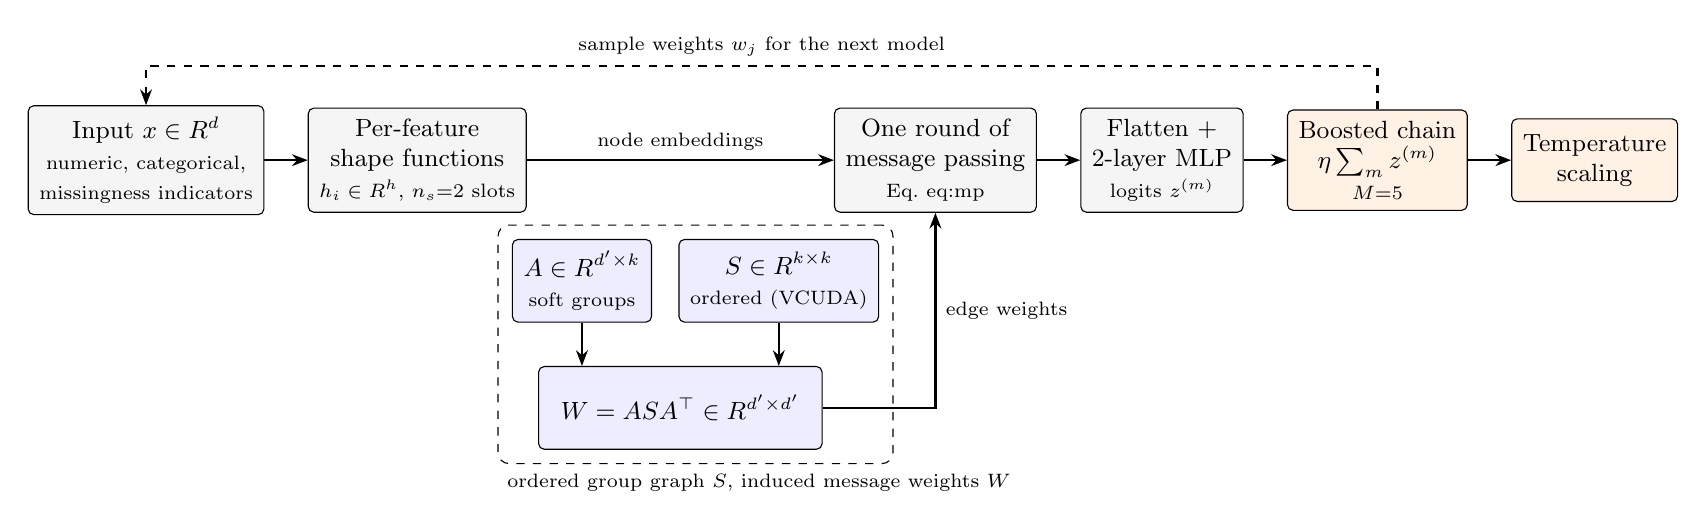
\begin{tikzpicture}[
  box/.style={draw, rounded corners=2pt, align=center, font=\small, minimum height=1.05cm, inner sep=4pt},
  dag/.style={box, fill=blue!7},
  net/.style={box, fill=gray!8},
  ens/.style={box, fill=orange!10},
  arr/.style={-{Stealth[length=2mm]}, thick}]
% main row
\node[net] (x) {Input $x\in\R^d$\\{\scriptsize numeric, categorical,}\\{\scriptsize missingness indicators}};
\node[net, right=0.55cm of x] (vsf) {Per-feature\\shape functions\\{\scriptsize $h_i\in\R^{h}$, $n_s{=}2$ slots}};
\node[net, right=3.9cm of vsf] (mp) {One round of\\message passing\\{\scriptsize Eq.~\eqref{eq:mp}}};
\node[net, right=0.55cm of mp] (head) {Flatten +\\2-layer MLP\\{\scriptsize logits $z^{(m)}$}};
\node[ens, right=0.55cm of head] (boost) {Boosted chain\\$\eta\sum_m z^{(m)}$\\{\scriptsize $M{=}5$}};
\node[ens, right=0.55cm of boost] (cal) {Temperature\\scaling};
% DAG block below
\coordinate (mid) at ($(vsf.east)!0.5!(mp.west)$);
\node[dag, below=1.0cm of mid, xshift=-1.25cm] (A) {$A\in\R^{d'\times k}$\\{\scriptsize soft groups}};
\node[dag, below=1.0cm of mid, xshift=1.25cm] (S) {$S\in\R^{k\times k}$\\{\scriptsize ordered (VCUDA)}};
\node[dag, below=0.55cm of $(A.south)!0.5!(S.south)$, minimum width=3.6cm] (W) {$W=ASA\T\in\R^{d'\times d'}$};
\node[draw, dashed, rounded corners, fit=(A)(S)(W), inner sep=5pt, label={[font=\scriptsize, anchor=north west]south west:ordered group graph $S$, induced message weights $W$}] (dagbox) {};
% arrows
\draw[arr] (x) -- (vsf);
\draw[arr] (vsf) -- node[above, font=\scriptsize] {node embeddings} (mp);
\draw[arr] (A.south) -- (A.south |- W.north);
\draw[arr] (S.south) -- (S.south |- W.north);
\draw[arr] (W.east) -| node[pos=0.75, right, font=\scriptsize] {edge weights} (mp.south);
\draw[arr] (mp) -- (head);
\draw[arr] (head) -- (boost);
\draw[arr] (boost) -- (cal);
\draw[arr, dashed] (boost.north) -- ++(0,0.55) -| node[pos=0.25, above, font=\scriptsize] {sample weights $w_j$ for the next model} (x.north);
\end{tikzpicture}}
\caption{The \Cabin{} pipeline. Features are embedded by private shape functions, softly assigned to $k$ groups by $A$, and connected through a group graph $S$ with a learned priority order; the induced message weights $W=ASA\T$ drive one round of message passing before a small MLP head. Five such networks form a boosted chain whose accumulated logits are temperature-scaled. The routing parameters ($A$, $\pi$, $E$) train only in the joint phase (\S\ref{sec:training}).}
\label{fig:pipeline}
\end{figure}
We consider classification with $n$ samples, $d$ input features and $C$ classes; every symbol is defined where it is introduced, and Table~\ref{tab:notation} (Appendix~\ref{app:method}) recaps them for reference. Figure~\ref{fig:pipeline} gives an overview; Appendices~\ref{app:design} and~\ref{app:hyper} give the design comparisons and every hyperparameter.

\subsection{Factored routing matrix}
\label{sec:factored}
A full feature-level routing matrix $W\in\R^{d\times d}$ has two problems on tabular data. An acyclicity constraint on it costs $O(d^3)$ per evaluation, and near-duplicate features force arbitrary orderings between variables that carry the same information. We factor it as
\begin{equation}
W = A\,S\,A\T,\qquad A=\mathrm{softmax}_{\text{row}}(A_{\text{raw}})\in\R^{d'\times k},\quad S\in\R^{k\times k},
\label{eq:factored}
\end{equation}
where $d'$ is the number of graph nodes (two per feature, \S\ref{sec:mp}), row $i$ of $A$ is the soft membership of node $i$ in $k$ groups and $S$ is a graph between groups. Correlated features can share a group, and directed structure lives in $S$, so the ordering acts on the $k\times k$ group matrix at a cost independent of $d$. The feature-level matrix $W$ is \emph{not} a DAG: with soft assignments, nodes that share a group exchange messages in both directions. Below, ``the learned graph'' refers to $(A,S)$ and the induced $W$, not to a feature-level causal DAG. We use $k=32$, fixed in development, where it beat auto-$k=\mathrm{clip}(\lfloor d/3\rfloor,2,64)$ on TabArena (Appendix~\ref{app:bench}); on CC18 with a fixed seed, any $k$ from 4 to 64 and auto-$k$ are within one point of it, none significantly (Appendix~\ref{sec:sensitivity}).

\subsection{Ordered group graph}
\label{sec:vcuda}
We parameterize $S$ with VCUDA \citep{hoang2024vcuda}: learnable priority scores $\pi\in\R^k$ and edge logits $E\in\R^{k\times k}$ give
\begin{equation}
S_{ab} = e_{ab}\, \sigma\!\left(\frac{\pi_b-\pi_a}{\tau_\pi}\right),\quad
e_{ab} = \begin{cases}
\mathrm{GumbelSigmoid}(E_{ab};\tau_E) & \text{(training)},\\
\mathbb{1}\!\left[\sigma(E_{ab}/\tau_E)>\tfrac12\right] & \text{(evaluation)},
\end{cases}
\label{eq:vcuda}
\end{equation}
with $e_{aa}=0$, $\sigma$ the logistic sigmoid and $\mathrm{GumbelSigmoid}$ a differentiable relaxed Bernoulli sample \citep{jang2017gumbel}. The edge indicator $e_{ab}$ gates a possible message from group $a$ to group $b$, and the priority sigmoid down-weights messages that go against the learned order. As $\tau_\pi\to0$ the sigmoid becomes a hard order and $S$ a DAG; at the finite $\tau_\pi=0.3$ we use, a reverse edge keeps a small nonzero weight, so strictly $S$ is a soft ordered relaxation of a DAG rather than a DAG, and no acyclicity penalty is used. The priorities set the direction of every edge, so directions in $S$ are a computation order, not evidence of causal direction; \S\ref{sec:structure} shows that on real data trained and untrained directions are not distinguishable by their asymmetry. A sparsity penalty $\lambda_s\|S\|_1$, $\lambda_s = 0.05+0.001\,d$, is applied during the joint phase; its growth with $d$ is inherited from earlier versions in which the routing was a $d\times d$ matrix.

\subsection{Message passing and feature representation}
\label{sec:mp}
Each numerical feature is embedded by a private two-layer shape function \citep{agarwal2021nam} into $n_s=2$ slots of dimension $32$ (the encodings $h_i$ of Eq.~\eqref{eq:mp}), so the graph has $d'=2d$ nodes; we call this a vector-valued shape function (VSF). Unlike a shared projection, it gives each feature its own nonlinear transformation before message passing, and the slots let a feature expose several complementary signals to the graph while each node stays tied to a single input variable. We set the dimension and $n_s$ on the development datasets (\S\ref{sec:protocol}). Categorical features use entity embeddings and missing values get indicator features (Appendix~\ref{app:hyper}). One round of Eq.~\eqref{eq:mp} with weights $W=ASA\T$ and edge dropout $0.2$ feeds a two-layer ReLU MLP on the $d'$ flattened embeddings.

\subsection{Training}
\label{sec:training}
We train each network with AdamW \citep{loshchilov2019adamw}, batch size 32, label smoothing $0.1$ \citep{szegedy2016rethinking} and 20\% of the training set held out for validation, in three phases. The \emph{warmup} (20 epochs) trains the encoders and the head with the routing parameters $(A_{\text{raw}},\pi,E)$ frozen at their random initialization, so that the routing starts to move only once the node embeddings carry signal; the \emph{joint} phase (100 epochs) trains all parameters, the routing parameters at a larger learning rate ($5\cdot10^{-3}$ vs $10^{-3}$) and with the sparsity penalty; the \emph{finetune} phase (30 epochs) freezes the routing again and adapts the rest of the network to it, with a tenth of the learning rate and early stopping. The weights with the lowest validation loss are restored at the end. Since tracking starts at the first epoch, the restored weights can predate routing training (\S\ref{sec:structure} measures how often).

\subsection{Boosted ensemble}
\label{sec:boosting}
We train $M=5$ networks sequentially (three are within seed noise of five, Appendix~\ref{sec:sensitivity}) and accumulate their logits with shrinkage $\eta=0.1$, the usual small step of gradient boosting \citep{friedman2001greedy}. After each model, training samples are reweighted by $w_j=\min\big(1+\alpha(1-p_{j,y_j}),\,3\big)$, where $p_{j,y_j}$ is the current ensemble probability of the true class: the next network focuses on the samples the ensemble gets wrong, and the cap at 3 keeps a few hard or mislabeled samples from dominating it. The strength $\alpha=2\,c_d\,c_n/\sqrt{C/2}$ grows with $d$ and $n$ through factors $c_d\in[0.3,1.2]$ (in $\log d$) and $c_n\in[0.5,1.5]$ (in $\sqrt n$) and shrinks with $C$ (exact form in Appendix~\ref{app:hyper}). A final temperature fitted on training logits leaves predictions unchanged. Other constants (temperatures, learning rates, epochs) were fixed in development, not tuned; Appendix~\ref{app:hyper} gives their origin.

% ============================================================================
\section{Experimental Protocol}
\label{sec:protocol}

\paragraph{Benchmarks.}
OpenML-CC18 \citep{bischl2021openml} contains 72 classification datasets. With a limit of one hour per fit, we compare methods on the \NCCtasks{} datasets where every method finished ($n$ from 500 to $5{,}620$, $d$ from 4 to 856, 2 to 19 classes), with 5-fold stratified cross-validation and default hyperparameters. Design choices and defaults were set on \emph{Dev8}, eight development datasets of which seven are in CC18 (Appendix~\ref{app:design}), so CC18 is not a held-out test of them. The largely held-out evaluation is TabArena \citep{erickson2025tabarena}: \TAdatasets{} classification datasets, \TAnotCC{} of them outside CC18, with its own protocol and baselines.

\paragraph{Statistics and seeds.}
We test paired differences with the Wilcoxon signed-rank test \citep{demsar2006statistical}, always with the \emph{dataset} as the unit: on real data, differences are averaged over folds before testing; on synthetic data, over the settings that share a random SCM. We treat effects below the seed noise floor (about half a point on the mean, Appendix~\ref{sec:sensitivity}) as not established. All runs of \S\ref{sec:when} and \S\ref{sec:structure} are new, with a fixed seed and folds 0--2 of the baseline splits.

% ============================================================================
\section{Results}
\label{sec:results}

\begin{table}[t]
\centering
\caption{Results with default hyperparameters. CC18 (\NCCtasks{} datasets): mean accuracy, its standard deviation $\sigma$ across datasets, average rank, strict wins. TabArena (\TAdatasets{} datasets): ELO, rank among \TAN{} methods (Table~\ref{tab:tabarena}), win rate.}
\label{tab:cc18}
\small
\setlength{\tabcolsep}{5pt}
\begin{tabular}{@{}llccccccc@{}}
\toprule
& & \multicolumn{4}{c}{CC18} & \multicolumn{3}{c}{TabArena} \\
\cmidrule(lr){3-6}\cmidrule(l){7-9}
Method & Type & Acc. & $\sigma$ & Rank & Wins & ELO & Rank & Win \% \\
\midrule
\inputtable{generated/table_main_results.tex}
\bottomrule
\end{tabular}

\vspace{8pt}
\caption{\Cabin{} minus LightGBM (points) on the datasets of Table~\ref{tab:cc18}.}
\label{tab:lgb}
\setlength{\tabcolsep}{5pt}
\begin{tabular}{@{}lcccccc@{}}
\toprule
\inputtable{generated/table_lightgbm_bins_wide.tex}
\bottomrule
\end{tabular}
\end{table}

\paragraph{CC18.}
Table~\ref{tab:cc18} compares \Cabin{} with tree-based and neural methods trained from scratch, and with the pre-trained TabICL as a foundation-model reference. Among methods trained from scratch, \Cabin{} has the best mean accuracy and average rank; it is \CabinVsTabMDelta{} points above TabM (nominal \CabinVsTabMPe{}, below the seed noise floor), and \CabinVsCatBoostDelta{} and \CabinVsLightGBMDelta{} points above CatBoost and LightGBM (\CabinVsCatBoostPe{} and \CabinVsLightGBMPe{}). With tuning, the ranking could change. On TabArena (Table~\ref{tab:cc18}; all methods in Table~\ref{tab:tabarena}), \Cabin{} reaches an ELO of \TAcabin{}, rank \TAcabinRank{} of \TAN{}, above every method trained from scratch (CatBoost \TAcatboost{}); the six methods above it are pre-trained in-context learners: the defaults transfer beyond Dev8.


\paragraph{Where \Cabin{} gains.}
Against LightGBM (Table~\ref{tab:lgb}), the advantage of \Cabin{} is largest on small datasets ($n<1{,}000$: \LGBNaDelta{} points, better on \LGBNaWins{}) and on low-dimensional ones ($d<20$: \LGBDaDelta{}, \LGBDaWins{}), and shrinks as $n$ grows (\LGBNbDelta{} for $1{,}000\le n<5{,}000$): \Cabin{} acts as a data-efficient neural model, though this breakdown does not isolate the graph.


\begin{table}[t]
\centering
\caption{Cumulative construction of \Cabin{} on the \CumN{} CC18 datasets common to all steps (linear-embedding pipeline). $\Delta_s$, $\Delta_t$: gain of the step and total gain (points); wins: datasets improved by the step; $p$: Wilcoxon test of the step.}
\label{tab:cumulative}
\small
\setlength{\tabcolsep}{4pt}
\begin{tabular}{@{}rlccccc>{\hspace{4pt}}l@{}}
\toprule
\# & Component & Acc. & $\Delta_s$ & $\Delta_t$ & Wins & $p$ & Purpose \\
\midrule
\inputtable{generated/table_cumulative_wide.tex}
\bottomrule
\end{tabular}
\end{table}
\paragraph{Design study and sensitivity.}
Table~\ref{tab:cumulative} builds \Cabin{} one step at a time (alternatives for seven design dimensions in Appendix~\ref{app:design}). Most of the gain comes from regularization and boosting; graph-specific steps (end-to-end routing, factoring) have small accuracy effects but make the model scale with $d$, and a second round of message passing hurts (\DFourKtwo{}). Varying one hyperparameter at a time on \SensTasks{} CC18 datasets (Appendix~\ref{sec:sensitivity}), no setting of the number of groups, edge dropout or label smoothing departs from the default by more than the seed noise floor. That the number of groups does not matter is a first hint that accuracy may not depend on the graph, which we now test.

% ============================================================================
\section{When Does the Feature Graph Help?}
\label{sec:when}

We now test the three explanations of \S\ref{sec:intro}: missing structure in the data, an architecture that cannot use a graph, or end-to-end training that does not find one. The true graph is unknown on real data, so a synthetic SCM with controlled interactions first tests the architecture and the training and yields predictions (\S\ref{sec:when-synth}); we check them on CC18 and ask, with an interaction proxy, whether CC18 has the structure a correct graph exploits (\S\ref{sec:when-real}).

\paragraph{Routing substitutions.}
\label{sec:substitutions}
Table~\ref{tab:routings} lists the routings we substitute for $W$ in Eq.~\eqref{eq:mp}. All share the network, the training schedule, the seed and the restore rule of \Cabin{}, and substituted routings stay fixed in training. As $W$ is unnormalized, denser routing also sums more messages. Because the restore rule can return a warmup checkpoint (\S\ref{sec:training}), the default routing may still be at its initialization (\LowSingleWarmupRestore{}\% and \HighSingleWarmupRestore{}\% of the low- and high-dimensional single networks on CC18, \S\ref{sec:when-real}).

\begin{table}[t]
\centering
\caption{Routings substituted for $W$ in Eq.~\eqref{eq:mp} and the question each answers. $^\ast$Synthetic only.}
\label{tab:routings}
\small
\begin{tabular}{@{}>{\raggedright}p{2.25cm}>{\raggedright}p{4.6cm}>{\raggedright\arraybackslash}p{7.45cm}@{}}
\toprule
Routing & Question & Message weights $W$ \\
\midrule
Default & Does end-to-end learning help? & $ASA\T$ of \S\ref{sec:method}, $(A,S)$ trained in the joint phase \\
None & Baseline any graph must beat & $W=0$ \\
Dense random & Is mixing features enough? & $(A,\pi,E)$ frozen at init.: dense, data-independent \\
True$^\ast$ & Can a correct graph help? & $G\otimes\mathbf{1}_{n_s\times n_s}$, $G$ the generating DAG on the inputs \\
Estimated & Is a two-stage estimate better? & Before training, $j$'s top-3 split-gain features in a LightGBM \citep{ke2017lightgbm} regressor of $x_j$ (100 trees, 8 leaves; 3: the synthetic degree), symmetrized: a moral-graph estimate \\
Sparse random & Sparsity, or the edges? & Random, edge count of True or Estimated \\
\bottomrule
\end{tabular}
\end{table}

\paragraph{Additive head (diagnostic).} The MLP head of \Cabin{} sees all node encodings at once, so it can model feature interactions without any message, and a graph may be unnecessary simply because the head does its work. As a diagnostic we therefore also use an additive head, a small MLP per node with logits summed over nodes, under which features can only interact through messages.

\subsection{A synthetic SCM with tunable interactions}
\label{sec:when-synth}

\paragraph{Generator.}
The generator must vary the factors that real datasets fix: the dimension, the sample size and how much of the signal comes from interactions, which a graph could route but an additive model cannot capture. We sample a DAG over $d$ variables by including each edge $j\to i$, $j>i$, independently with probability $p$, and generate the nodes in reverse index order. A node without parents is $\mathcal N(0,1)$; a node $i$ with parent set $P_i$ is
\begin{equation}
\begin{gathered}
a_i = z\Big(\textstyle\sum_{j\in P_i} w_{ji}\, f_{ji}(x_j)\Big),\qquad
b_i = z\Big(\textstyle\sum_{j<l,\ j,l\in P_i} c_{jl}\, g_{ji}(x_j)\, g_{li}(x_l)\Big),\\
x_i = z\Big(\sqrt{1-\lambda}\;a_i + \sqrt{\lambda}\;b_i + \varepsilon_i\Big),
\end{gathered}
\label{eq:scm}
\end{equation}
where $\varepsilon_i\sim\mathcal N(0,0.5^2)$, $z(\cdot)$ standardizes over the generated sample (a generator step, not available to the learner), $w$ and $c$ are uniform on $\pm[0.3,1]$ (bounded away from zero), and $b_i=0$ when $|P_i|<2$; at $\lambda=1$ a single-parent node is then independent of its parent, so the true graph is not faithful there. The parameter $\lambda$ moves the mechanisms from purely additive ($\lambda=0$) to purely pairwise interactions between co-parents ($\lambda=1$). The target is the node with the most parents among those with at least two parents and one child (lowest index on ties), binned into three classes at training-set terciles; it is removed from the inputs, and the \emph{true} graph is the induced subgraph over the remaining $d-1$ features (the generating structure, not the best routing: marginalizing the target adds edges). Predictive information comes from the target's parents, children and co-parents (its Markov blanket), and interactions among them make graph-restricted messages potentially useful. We use two regimes, which the real-data study of \S\ref{sec:when-real} mirrors:
\begin{itemize}
\item \emph{Low dimension}, like most CC18 datasets: $d\in\{10,20\}$, $p=0.3$, $f=\tanh$, $g$ the identity; $n=2{,}000$ with $\lambda\in\{0,0.25,0.5,0.75,1\}$, and $n=10^4$ with $\lambda\in\{0,1\}$.
\item \emph{High dimension} with few samples, where a sparse graph should matter most as a prior: $d\in\{50,100\}$, $p=4/d$ (an expected degree of four at every $d$), $n\in\{500,1000\}$, $\lambda\in\{0,1\}$; each $f_{ji}$ and $g_{ji}$ is one of seven nonlinear mechanisms with random scale and offset (Appendix~\ref{app:when}), in the spirit of tabular foundation-model priors \citep{hollmann2023tabpfn}.
\end{itemize}
Each $d$ uses five random SCMs, shared across $n$ and $\lambda$, and fresh test samples (2,000 in low and 5,000 in high dimension). \emph{The unit of every test is the SCM}: paired differences are averaged over the $n$ and $\lambda$ settings that share an SCM (or over $n$ only when a test is restricted to one $\lambda$), giving ten units per regime. As references we report LightGBM, LightGBM with stumps (an additive model, which measures how much interactions matter; Appendix~\ref{app:when}) and LightGBM restricted to the true Markov blanket of the target (an oracle that measures how much feature selection matters).

\begin{table}[t]
\centering
\caption{Synthetic SCM of Eq.~\eqref{eq:scm}: test accuracy (three classes, chance $\approx0.333$) of a single network with the MLP head and each routing (Table~\ref{tab:routings}), averaged over two values of $d$ and five SCMs. \emph{LGBM-MB}: LightGBM on the true Markov blanket of the target (an oracle). Best non-oracle model in bold; --: not run ($n=10^4$ serves the additive head).}
\label{tab:when-synth}
\small
\setlength{\tabcolsep}{4pt}
\begin{tabular}{@{}lcccccccc@{}}
\toprule
Regime & $\lambda$ & None & Dense & Default & True & Estimated & LightGBM & LGBM-MB \\
\midrule
\inputtable{generated/table_struct_synth.tex}
\bottomrule
\end{tabular}
\end{table}

\begin{figure}[t]
\centering
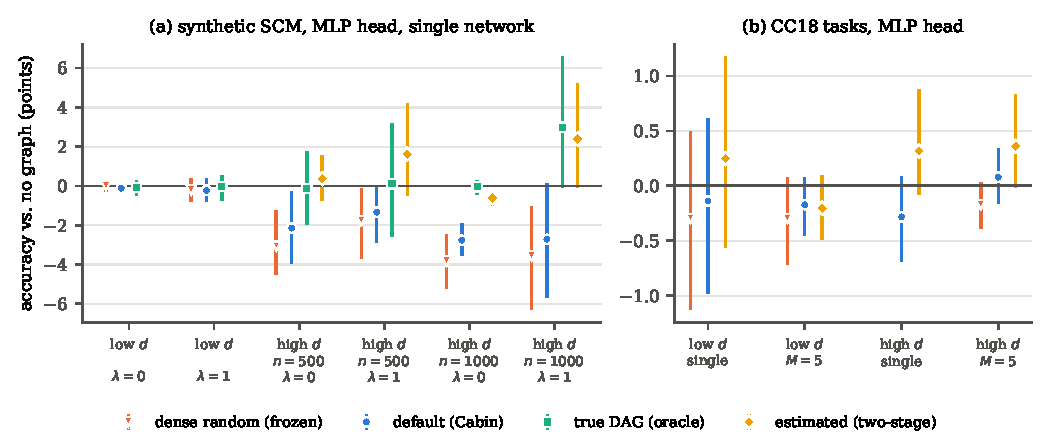
\includegraphics[width=\textwidth]{generated/fig_structure.pdf}
\caption{Accuracy difference to the same network without graph (points; mean and 95\% bootstrap interval over SCMs in (a) and datasets in (b)). (a) Synthetic SCM (Table~\ref{tab:when-synth}): with few features the graph choice does not matter; with many features dense random routing hurts, the true graph is most useful in the interaction settings, and the default routing stays close to dense random routing. (b) CC18 (Table~\ref{tab:when-real}): no effect on low-dimensional datasets; on high-dimensional ones the estimated graph is the furthest above zero.}
\label{fig:when}
\end{figure}

\paragraph{Low dimension: the graph choice does not matter.}
With $d\le20$, the four routings are within \SynLowSpread{} points of each other at every $\lambda$ (Table~\ref{tab:when-synth}, Figure~\ref{fig:when}a). Over the \SynLowTrueNoneN{} low-dimensional SCMs at $n=2{,}000$, averaging over $\lambda$, the true graph differs from no graph by \SynLowTrueNone{} points (\SynLowTrueNonePe{}) and from a random graph by \SynLowTrueRand{} (\SynLowTrueRandPe{}); the default routing differs from no graph by \SynLowLearnNone{} (\SynLowLearnNonePe{}). The messages are not useless, however. With the additive head at $n=10^4$ and $\lambda=1$, where interactions can only come from messages, dense routing helps: dense random routing adds \SynBigAddRandNone{} points over no graph (\SynBigAddRandNonePe{}, \SynBigAddRandNoneWL{}), but the true graph is no better than the random one (\SynBigAddTrueRand{}, \SynBigAddTrueRandPe{}; Appendix~\ref{app:when}). With few features, dense routing connects almost every pair, so it expresses what the true graph can.

\paragraph{High dimension: dense random routing hurts, a correct graph can help.}
With $d\in\{50,100\}$ and $n\le1{,}000$, dense random routing is \SynHighRandNoneAbs{} points below no graph (\SynHighRandNoneWL{} SCMs, \SynHighRandNonePe{}): mixing every feature into every node mostly adds noise with few samples. The true graph avoids this loss and beats dense random routing by \SynHighTrueRandAbs{} points (\SynHighTrueRandWL{}, \SynHighTrueRandPe{}). Against no graph it is neutral when the mechanisms are additive (\SynHighTrueNoneLamZero{}, $\lambda=0$) and ahead with interactions, but not significantly with the MLP head (\SynHighTrueNoneLamOne{} at $\lambda=1$, \SynHighTrueNoneLamOnePe{}); with the additive head, where interactions must pass through messages, it adds \SynHighAddTrueNoneLamOne{} points at $\lambda=1$ (\SynHighAddTrueNoneLamOnePe{}). The no-graph network often restores an early single-class checkpoint (\SynHighEarlyRestore{}\% of runs), so the density-matched control is firmer.

\paragraph{Density versus edge identity.}
The sparse random controls matched to the true and estimated graphs are not detectably different from no graph (\SynHighRandTrueNone{} and \SynHighRandEstNone{} points, \SynHighRandTrueNonePe{} and \SynHighRandEstNonePe{}) and beat dense random routing (\SynHighRandTrueRandom{} and \SynHighRandEstRandom{}, \SynHighRandTrueRandomPe{} and \SynHighRandEstRandomPe{}): the loss of dense random routing is mostly an effect of density, or of the message scale that comes with it, which we do not separate. Edge identity still matters for the true graph, which beats its density-matched control by \SynHighTrueRandTrueAbs{} points (\SynHighTrueRandTrueWL{}, \SynHighTrueRandTruePe{}), \SynHighTrueRandTrueLamOneAbs{} at $\lambda=1$ (nominal \SynHighTrueRandTrueLamOnePe{}) and \SynHighAddTrueRandTrueLamOneAbs{} with the additive head at $\lambda=1$ (\SynHighAddTrueRandTrueLamOnePe{}). The estimated graph is ahead of its own control by a non-significant \SynHighEstRandEstAbs{} points (\SynHighEstRandEstPe{}): its advantage over dense random routing is mostly sparsity.

\paragraph{The default end-to-end procedure does not return a useful graph.}
The default routing is not significantly better than dense random routing (\SynHighLearnRand{} points, \SynHighLearnRandPe{}) and is worse than no graph (\SynHighLearnNone{}, \SynHighLearnNonePe{}). Two reasons lie in the training schedule. In \SynHighWarmupRestore{} of its \SynHighLearnedRuns{} runs the restored checkpoint predates routing training, returning the dense random routing. In the others, the joint phase starts from a dense random routing the network already adapted to during warmup. Fixes aimed at each reason (Appendix~\ref{app:when}) do not help at $\lambda=0$; learning the factored graph within the estimated skeleton beats the true graph at $\lambda=1$ (\SynHighSkelEstTrueLamOne{} points) but loses \SynHighSkelEstTrueLamZeroAbs{} at $\lambda=0$.

\paragraph{A separately estimated graph approaches the true graph.}
If joint learning is the problem, a graph estimated before training should do better. The two-stage estimated graph beats dense random routing by \SynHighEstRandAbs{} points (\SynHighEstRandPe{}) and the default routing by \SynHighEstLearnAbs{} (\SynHighEstLearnPe{}), and is not detectably different from the true graph (\SynHighTrueEst{} points, \SynHighTrueEstPe{}; this does not establish equivalence). Ranked by split gain, its candidate edges recover the true skeleton with a mean ROC AUC of \SynEstAucSkel{} (co-parent edges, which a regression screen should find, count as errors). Like the true graph, it gains over no graph only with interactions, significantly with the additive head (\SynHighAddEstNoneLamOne{} at $\lambda=1$, \SynHighAddEstNoneLamOnePe{}). In this SCM, estimating a sparse predictive graph before training thus reaches true-graph accuracy far better than joint learning, though much of the gain is sparsity.

\paragraph{In high dimension, feature selection matters more than wiring.}
At $\lambda=1$, LightGBM is \SynHighLgbTrueLamOneAbs{} points above the network with the true graph, and LightGBM restricted to the true Markov blanket is \SynHighMbLgbLamOneAbs{} points above LightGBM on all features (\SynHighMbLgbLamOnePe{}), as stochastic feature gates \citep{yamada2020feature} also suggest (Appendix~\ref{app:when}).

\paragraph{Predictions for real data.} The architecture can exploit a correct graph, but training does not find it. The SCM predicts that with few features the graph does not matter, that with many features dense random routing hurts but sparse graphs do not, and that the default routing matches controls.

\subsection{Real data: consistent with the predictions}
\label{sec:when-real}

\begin{table}[t]
\centering
\caption{Graph substitutions on CC18 (folds 0--2, seed 42). \emph{Default}: accuracy of \Cabin{}; other columns: differences in points between the routings of Table~\ref{tab:routings} (\emph{Sparse}: random symmetric graph with the edge count of the estimated graph). $^{*}$: $p<0.05$, $^{**}$: $p<0.01$, Wilcoxon over datasets (fold-averaged). --: not run; \emph{cnae-9} excluded (Appendix~\ref{sec:when-cnae}).}
\label{tab:when-real}
\small
\setlength{\tabcolsep}{4pt}
\begin{tabular}{@{}llcccccccc@{}}
\toprule
& & & \multicolumn{4}{c}{column $-$ Default} & \multicolumn{2}{c}{Est.\ $-$ column} \\
\cmidrule(lr){4-7}\cmidrule(lr){8-9}
Datasets & Model & Default & Dense & Sparse & None & Est. & Sparse & None \\
\midrule
\inputtable{generated/table_struct_real.tex}
\bottomrule
\end{tabular}
\end{table}

We use the \RealNLow{} CC18 datasets of the sensitivity analysis ($d\le\RealLowDMax{}$, $n<5{,}000$) and \RealNHigh{} high-dimensional CC18 datasets with $\RealHighDMin{}\le d\le\RealHighDMax{}$ (listed in Appendix~\ref{app:when}), each on three folds, as a single network and as the five-model ensemble.

\paragraph{Low-dimensional datasets.}
On the \RealNLow{} low-dimensional datasets, as predicted, no substitution, sparse control included, changes accuracy significantly for single networks or ensembles (Table~\ref{tab:when-real}).

\paragraph{High-dimensional datasets.}
On the \RealNHigh{} high-dimensional datasets the signs match the predictions, with small effects. In the ensemble, the dense random graph is worse than the default (\RealHighEnsRandomLearned{}, \RealHighEnsRandomLearnedPe{}), and the estimated graph is better than dense random routing (\RealHighEnsEstimatedRandom{}, \RealHighEnsEstimatedRandomPe{}) but only \RealHighEnsEstimatedNone{} points above no graph (\RealHighEnsEstimatedNonePe{}). The sparse control removes this advantage: the estimated graph is only \RealHighEnsEstimatedSparse{} points above it in the ensemble (\RealHighEnsEstimatedSparsePe{}), so its gain over dense random routing is mostly sparsity rather than its particular edges, as in the synthetic SCM. These effects are tenths of a point, on ten datasets and one seed.

\paragraph{The messages are used, but the default routing is not special.}
The trained network relies on its messages: setting $W=0$ only at test time lowers accuracy by \WZeroDrop{} points on average (median \WZeroDropMedian{}). But networks trained from scratch with a random graph or none adapt to it equally well: over all \RealPoolEnsNoneLearnedN{} datasets, the ensemble without graph is \RealPoolEnsNoneLearned{} points from the default (\RealPoolEnsNoneLearnedPe{}): the ranking of Table~\ref{tab:cc18} is not evidence for the graph.

\paragraph{Do benchmark datasets have the structure?}
\label{sec:when-interact}
Most CC18 datasets are low-dimensional, where the synthetic graph choice did not matter. As a proxy for interactions, we compare LightGBM with its stump-only additive version (\S\ref{sec:when-synth}). Over the \IntNTasks{} CC18 datasets of Table~\ref{tab:cc18}, the median gain of the full model is \IntMedian{} points; only \IntNGapOne{} datasets gain more than one point, and on \IntNNeg{} the additive model is better. Across the \RealNLow{} low-dimensional datasets, the proxy correlates with the default routing's gain over no routing for the diagnostic additive head (Spearman $\rho=\AddFtRho{}$, nominal \AddFtRhoPe{}), not for the MLP head ($\rho=\MlpLearnedRho{}$), which models interactions.

% ============================================================================
\section{What Does the Learned Graph Encode?}
\label{sec:structure}

Recovery is not expected from a prediction loss; we check whether it happens (Appendices~\ref{sec:synthetic} and~\ref{sec:realdags}).

\paragraph{Group-level structure on synthetic DAGs.}
We use the usual benchmark of differentiable structure learning \citep{zheng2018dags}: Erd\H{o}s--R\'enyi DAGs with $d\in\{10,20,50\}$ and linear or $\tanh$ mechanisms. We score $S$ against the true DAG collapsed to the learned groups (auto-$k$): the skeleton F1 is \SynAutoSkelGrp{}, but collapsing makes the target graph dense: a random $S$ with the same number of edges already reaches \SynRandSkelGrp{}. The learned $S$ is above this chance level for the skeleton (\SynRandSkelPe{} over \SynRandN{} SCMs) but not for directions (directed F1 \SynAutoDirGrp{} vs.\ \SynRandDirGrp{}, \SynRandDirPe{}).

\paragraph{Two limits on real data.}
We retrain the first network on the \DagN{} datasets of Table~\ref{tab:cc18}. First, in \DagBaseUntrained{}\% of them the restored checkpoint predates routing training, so the returned routing is at its random initialization. Changing the restore rule does not fix this: validation loss rises during the joint phase while accuracy stays flat, and restoring only post-routing checkpoints changes accuracy by \SensFixSeedsDelta{} points on the \SensTasks{} datasets of \S\ref{sec:results} (\SensFixSeedsN{} seeds, \SensFixSeedsPe{}). Second, $S$ is strongly asymmetric, trained or not (asymmetry \DagAsymUntrained{} untrained vs.\ \DagAsymTrained{} trained, max 2), so it cannot show a learned order (\S\ref{sec:vcuda}).

% ============================================================================
\section{Conclusion}
\label{sec:conclusion}

We asked whether graph-informed tabular models owe their accuracy to their graph. Answering required a model worth testing: \Cabin{}, with defaults set on Dev8, has the best mean accuracy on CC18 and the highest TabArena ELO among the methods trained from scratch that we evaluate. With \Cabin{} as a test bed, we tested three reasons a feature graph might not help. The architecture is not the obstacle: in the high-dimensional SCM, a correct graph beats density-matched random routing. The data are a partial obstacle: many CC18 datasets have few features and weak interactions. The main obstacle is learning: the end-to-end routing of \Cabin{} is not more useful than controls, while in the high-dimensional SCM a separately estimated graph is not detectably worse than the true one, mostly by being sparse. Message passing is a real source of accuracy when the graph is correct and sparse; learning such graphs is where graph-informed models can gain most.

\paragraph{Outlook.} These results point to concrete next steps. First, decouple structure estimation from prediction: a cheap two-stage graph already beats the default routing by \SynHighEstLearnAbs{} points in the high-dimensional SCM, and stronger structure-learning methods can be plugged in the same way. Second, let the routing actually train: schedules in which the routing is learned before the network adapts to a random one are a direct target, since the restored routing is untrained in \DagBaseUntrained{}\% of CC18 datasets. Third, combine routing with feature selection: in high dimension, an oracle restricted to the Markov blanket of the target gains \SynHighMbLgbLamOneAbs{} points, so a graph that also selects features could add to what routing alone brings. Finally, our protocol of substituting routings in a fixed network and testing them on an SCM with tunable interactions applies to any graph-informed model, and can serve as a standard check that a learned graph earns its place.

\paragraph{Limitations.} Learned graphs on real data support no causal claim (\S\ref{sec:structure}); the SCM has no latent confounding; we test neither edge orientation nor interventions.

% Acknowledgments---Will not appear in anonymized version
\acks{Withheld for review.}

\bibliography{references}

\appendix
% ============================================================================
\section{Method Details}
\label{app:method}

\begin{table}[t]
\centering
\caption{Notation recap (optional; every symbol is defined in the main text).}
\label{tab:notation}
\footnotesize
\setlength{\tabcolsep}{3pt}
\begin{tabular}{@{}ll@{\hspace{10pt}}ll@{}}
\toprule
$n,d,C$ & samples, input features, classes & $\pi\in\R^k,\ E\in\R^{k\times k}$ & priority scores, edge logits of $S$ \\
$n_s,\ d'=n_s d$ & slots per feature (2), graph nodes & $\tau_\pi,\ \tau_E$ & priority (0.3), edge (0.5) temperatures \\
$k$ & number of groups (32) & $h_i,\ \tilde h_i$ & node $i$ encoding, before/after messages \\
$A\in\R^{d'\times k}$ & soft node-to-group assignment & $M,\ \eta$ & ensemble size (5), shrinkage (0.1) \\
$S\in\R^{k\times k}$ & ordered group graph & $w_j,\ \alpha$ & sample weight, reweighting strength \\
$W=ASA\T$ & node message weights ($d'\times d'$) & & \\
\bottomrule
\end{tabular}
\end{table}



\paragraph{Optional extensions}
\label{sec:extensions}
The default model defines one global routing mechanism shared by all samples. We evaluate three exploratory extensions that are not part of the default recipe. \emph{MoE-DAG} learns $K=4$ group-level ordered graphs $S_1,\dots,S_K$ with a shared $A$ and a gating MLP $g(x)$, so that $W(x)=A\big(\sum_k \sigma(g_k(x))S_k\big)A\T$ varies per sample, following the intuition that predictive routing may vary across samples (inspired by work on local causal structure, \citealp{baumgartner2026disentangling}, but used here only as a predictive variant). \emph{Contrastive VSF} adds a supervised contrastive loss \citep{khosla2020supervised} ($\tau=0.5$, weight $0.5$) on the pre-message-passing embeddings. \emph{Annealed sparsity} splits $S=S_{\text{base}}+S_{\text{sparse}}$ and ramps an $\ell_1$ penalty on $S_{\text{sparse}}$ during the joint phase.

\paragraph{Worked example}
\label{sec:example}
As an idealized illustration of the parameterization, not a claim about what training recovers, consider $d=6$ features where $x_1,x_2$ are two noisy measurements of one quantity, $x_3,x_4$ of a second quantity caused by the first, and $x_5,x_6$ of a third caused by both, with $k=3$ and $n_s=1$ for simplicity. The parameterization can represent $A$ close to the hard assignment $\{x_1,x_2\}\mapsto 1$, $\{x_3,x_4\}\mapsto 2$, $\{x_5,x_6\}\mapsto 3$, priorities $\pi_1<\pi_2<\pi_3$, and edges $e_{12}=e_{13}=e_{23}=1$, so that
\[
S\approx\begin{pmatrix}0&1&1\\0&0&1\\0&0&0\end{pmatrix},\qquad
W=ASA\T\approx\begin{pmatrix}0&1&1\\0&0&1\\0&0&0\end{pmatrix}\otimes\begin{pmatrix}1&1\\1&1\end{pmatrix}.
\]
Message passing then sends both measurements of quantity 1 to every node of groups 2 and 3, and the nodes of group 3 receive from groups 1 and 2. The representation exposes three groups and a chain $1\to2\to3$ with a shortcut, rather than $6\cdot5=30$ possible feature-level edges, and the two near-duplicates $x_1,x_2$ need no order between them. Appendix~\ref{sec:synthetic} tests whether training recovers such structure: much of the grouped score is explained by the grouping itself, and directions are at chance.


% ============================================================================
\section{Design Study}
\label{app:design}
\label{sec:design}

\paragraph{Dev8.} The development suite of \S\ref{sec:protocol} consists of \emph{sonar}, \emph{cylinder-bands}, \emph{spambase}, \emph{steel-plates-fault}, \emph{mfeat-zernike}, \emph{segment}, \emph{semeion} and \emph{cnae-9}, evaluated with 5-fold cross-validation; all but \emph{sonar} belong to CC18. It mixes low- and high-dimensional datasets ($d$ up to 856).

\begin{table}[t]
\centering
\caption{Design dimensions on CC18 (5-fold CV, linear-embedding pipeline). Each block compares alternatives on the datasets where all of them finished ($n$); the selected option is in bold. $\Delta$: mean difference to the selected option in accuracy points; $p$: Wilcoxon signed-rank test against it.}
\label{tab:design}
\small
\begin{tabular}{@{}llccccl@{}}
\toprule
Dimension & Variant & Acc. & $\Delta$ & Rank & $p$ & \\
\midrule
\inputtable{generated/table_design.tex}
\bottomrule
\end{tabular}
\end{table}


Table~\ref{tab:design} compares the options for each design dimension and Table~\ref{tab:cumulative} builds \Cabin{} one step at a time.

\paragraph{D1: Graph learning.}
Learning the graph end to end with the predictor (SDCD, spectral-radius constraint) obtains the best average rank (\DOneSDCDRank{}) against the two-stage CASTLE (\DOneCastleRank{}) and GOLEM (\DOneGolemRank{}) pipelines, with a small accuracy gain (\DOneDeltaCastle{} points over CASTLE, \DOneCastlePe{}). End-to-end training lets the prediction loss shape the routing weights, which the factored routing matrix and boosting build on.

\paragraph{D2: Routing parameterization.}
The factored routing matrix $W=ASA\T$ obtains the best mean accuracy (\DTwoFactAcc{}) and rank (\DTwoFactRank{}) against the full $d\times d$ matrix (\DTwoFullAcc{}), block-diagonal regularization (\DTwoBlockAcc{}) and latent nodes (\DTwoLatentAcc{}). The gain over the full matrix is small (\DTwoDeltaFull{} points, \DTwoFullPe{}); its value is that the ordering or acyclicity mechanism acts on the $k\times k$ group matrix rather than the $d\times d$ feature matrix, and that the routing is inspectable at group level, at no accuracy cost.

\paragraph{D3: Acyclicity.}
Once the constraint acts on a $32\times32$ matrix, the mechanism barely matters: spectral radius, DP-DAG and VCUDA reach \DThreeSpectralAcc{}, \DThreeDPDAGAcc{} and \DThreeVCUDAAcc{} on \DThreeN{} datasets. DAGMA finished within the one-hour-per-job budget on only \DThreeDagmaN{} datasets (\DThreeDagmaAcc{} vs \DThreeDagmaVcudaAcc{} for VCUDA on the same datasets) and is omitted from the table. We select VCUDA because it needs no penalty schedule (its order is built into the parameterization).

\paragraph{D4: Message passing.}
A second or third round of message passing hurts consistently (\DFourKtwo{} and \DFourKthree{} points, \DFourKtwoPe{} for $K=2$): repeated propagation over an imperfect routing matrix blurs the signal more than it refines it.

\paragraph{D5: Feature representation.}
Replacing the shared linear embedding by per-feature VSF embeddings does not change accuracy: on the \VSFN{} datasets present in both pipelines, the VSF variant averages \VSFVsf{} against \VSFLin{} ($\Delta=\VSFDelta{}$ points, better on \VSFBetter{} and worse on \VSFWorse{} datasets, \VSFPe{}; the two use different folds, so this comparison is descriptive). We keep VSF because each node stays tied to a single input variable. Missingness indicators are neutral on average; RTDL periodic embeddings \citep{gorishniy2022embeddings} were unstable on high-dimensional datasets and did not help.

\paragraph{D6: Ensembling and temperature scaling.}
Boosting brings the second-largest gain of the construction (\CumEDelta{} points, \CumEWins{} datasets, Table~\ref{tab:cumulative}); a single model is \DSixSingle{} points below the full ensemble on \DSixN{} datasets. Adaptive reweighting (\CumFDelta{}) and temperature scaling (\CumGDelta{}) do not change accuracy; temperature scaling is a scalar rescaling of the logits and cannot change predicted classes; it is kept only for parity with the original pipeline, and because it is fitted on training logits we make no calibration claim. Regularization by label smoothing and edge dropout is the largest single step (\CumDDelta{} points, \CumDWins{} datasets).

\paragraph{D7: Beyond a single global routing mechanism.}
On the \NCCtasks{} datasets of Table~\ref{tab:cc18}, MoE-DAG and contrastive VSF change the mean accuracy by \DSevenMoEDelta{} and \DSevenConDelta{} points (neither significant: \CabinVsCabinMoEPe{} and \CabinVsCabinConPe{}), and annealed sparsity changes it by \DSevenAnnealDelta{} points. Given the seed-to-seed variability measured in \S\ref{sec:sensitivity}, we do not consider any of them an improvement and leave them out of the default recipe.

\paragraph{Overall.}
From CASTLE+CINN to \Cabin{}, mean accuracy goes from \CumStart{} to \CumEnd{} (\CumTotal{} points) on the \CumN{} datasets common to all steps. The steps that matter are regularization and boosting; the graph-specific steps (end-to-end training, factoring) are small in accuracy but make the routing mechanism scale with $d$ and be inspectable at group level.

\paragraph{Negative results.}
Besides the variants of Table~\ref{tab:design}, the following did not help during development and are documented, with their measured effects, in Appendix~\ref{app:negative}: reducing dimensionality before the routing mechanism (PCA: $-0.6$ to $-4.7$ points on Dev8; linear or attention-based grouping), reconstruction and denoising losses, self-supervised masked pre-training, replacing message passing by attention, pooled readouts, learnable edge weights after the DAG is fixed, Monte-Carlo sampling of the DAG at test time, pre-extracted DAGs from external discovery algorithms, and majority or out-of-bag voting instead of boosting.


% ============================================================================
\section{Additional Benchmark Results}
\label{app:bench}

\paragraph{Cost.}
On our hardware the median wall-clock time per fold is \TimeSingle{}\,s for a single network and \TimeEnsemble{}\,s for the five-model ensemble (runs were spread over different machines, so these are indicative). This is comparable to other neural methods and two to three orders of magnitude slower than LightGBM. Appendix~\ref{sec:sensitivity} shows that three boosted models give nearly the accuracy of five.

\begin{table}[h]
\centering
\caption{CC18 comparison of Table~\ref{tab:cc18} with the exploratory \Cabin{} variants of Appendix~\ref{sec:extensions} (rank among ten methods; \NCCtiesFull{} datasets have tied best methods). The variants are not used in any graph ablation.}
\label{tab:cc18full}
\small
\begin{tabular}{@{}llcccc@{}}
\toprule
Method & Type & Mean acc. & $\sigma$ & Rank & Wins \\
\midrule
\inputtable{generated/table_cc18_full.tex}
\bottomrule
\end{tabular}
\end{table}

\begin{table}[t]
\centering
\caption{TabArena classification leaderboard (default configurations, TabArena protocol). $^\dagger$Pre-trained on external synthetic corpora.}
\label{tab:tabarena}
\small
\begin{tabular}{@{}rlccc@{}}
\toprule
& Method & ELO & Avg.\ rank & Win rate (\%) \\
\midrule
\inputtable{generated/table_tabarena.tex}
\bottomrule
\end{tabular}
\end{table}

\paragraph{TabArena.}
On TabArena (Table~\ref{tab:tabarena}), with $k=32$, \Cabin{} reaches an ELO of \TAcabin{} (rank \TAcabinRank{} of \TAN{}), above every method trained from scratch, including CatBoost (\TAcatboost{}); the six methods above it are all pre-trained in-context learners. With auto-$k$, \Cabin{} drops to \TAautok{} (rank \TAautokRank{}). MoE-DAG and contrastive VSF were not run on TabArena.



\paragraph{When does \Cabin{} help?}
Against LightGBM (Table~\ref{tab:lgb}), the largest losses are on \LGBWorstaTask{} (\LGBWorstaDelta{}) and \LGBWorstbTask{} (\LGBWorstbDelta{}).


% ============================================================================
\section{Sensitivity and Routing Ablations}
\label{sec:sensitivity}

\begin{table}[t]
\centering
\caption{Sensitivity of a single \Cabin{} network (no ensemble) to one hyperparameter at a time, on \SensTasks{} CC18 datasets with $d\le 41$ and \SensFolds{} folds (\SensPairs{} dataset--fold pairs), same seed for all configurations; accuracies average over these pairs, while W/L counts datasets and $p$ is an Wilcoxon test over datasets after averaging fold differences. Defaults in bold. $\Delta$: mean difference to the default in accuracy points; W/L: pairs where the variant is better/worse; $p$: Wilcoxon test against the default.}
\label{tab:sensitivity}
\small
\begin{tabular}{@{}llcccc@{}}
\toprule
Hyperparameter & Value & Acc. & $\Delta$ & W/L & $p$ \\
\midrule
\inputtable{generated/table_sensitivity.tex}
\bottomrule
\end{tabular}
\end{table}

\paragraph{Setup.}
To measure how much the defaults matter we vary one hyperparameter at a time around the default configuration on \SensTasks{} CC18 datasets with up to 41 features and fewer than 5,000 samples (larger ones are too costly to sweep), using folds 0--2 of the baseline-comparison splits. We train a single network per configuration so that the effect is not diluted by the ensemble, and use the same seed for every configuration so that differences are paired. Two additional runs of the default with different seeds give the noise floor, and a ten-model ensemble scored after 1, 3, 5 and 10 models gives the effect of the ensemble size. All results are in Table~\ref{tab:sensitivity}.

\paragraph{Noise floor.}
Changing only the seed moves individual accuracies by \SensSeedSd{} points on average (standard deviation across seeds) and the mean over all pairs by up to \SensSeedMeanSpread{} points, with no consistent seed effect. Differences smaller than this should not be read as effects; of the hyperparameter changes below, only $k=8$ exceeds it, and barely.

\paragraph{Number of groups $k$.}
On these small and medium datasets, every $k$ from 4 to 16 is slightly better than the default 32 (\SenskFourDelta{}, \SenskEightDelta{}, \SenskOneSixDelta{} points), as is auto-$k$ (\SenskautoDelta{}), while $k=64$ is equivalent (\SenskSixFourDelta{}). None of these differences is significant at the dataset level (smallest: \SenskEightPe{} for $k=8$). The submitted explanation that auto-$k$ lost on TabArena because low-dimensional datasets fall ``below 8 groups'' is not supported: on the \SensLowDN{} datasets with $d<12$, $k=4$ and $k=8$ change accuracy by \SensLowDkFourDelta{} and \SensLowDkEightDelta{} points. The accuracy is therefore flat in $k$ to within about one point, and $k$ mainly controls the granularity of the group routing (\S\ref{sec:synthetic}).

\paragraph{Regularization.}
Edge dropout and label smoothing have small effects in the range we tested (all within $\pm$\,0.3 points, none significant); single-network accuracy is not sensitive to them, and their benefit in Table~\ref{tab:cumulative} comes with the ensemble.

\paragraph{Ensemble size.}
Over \SensEnsN{} dataset--fold pairs, accuracy goes from \SensEnsOne{} with one network to \SensEnsThree{}, \SensEnsFive{} and \SensEnsOneZero{} with 3, 5 and 10. Three models are within \SensEnsThreeVsFive{} points of five, and ten add \SensEnsTenVsFive{}: $M=3$ is a reasonable choice when cost matters.

\paragraph{Routing ablations and the restore rule.}
The last two blocks of Table~\ref{tab:sensitivity} replace the default routing by the dense random routing it is initialized with (the routing parameters $(A,\pi,E)$ are frozen for the whole training) and remove message passing entirely ($W=0$, so each node keeps only its own encoding). Neither changes accuracy beyond the seed noise, for a single network (\SensranddagDelta{} and \SensnodagDelta{} points) or for the five-model ensemble (\SensranddagensFiveDelta{} and \SensnodagensFiveDelta{}). The many ties of the random-graph row come from the restore rule of \S\ref{sec:training}: when the restored checkpoint predates the joint phase, the default model already returns its initial routing weights (\S\ref{sec:realdags}). Fixing the rule does not help: allowing only finetune-phase checkpoints, so that the returned graph is always trained, changes accuracy by \SensfixrestoreDelta{} points in the seed-42 run of Table~\ref{tab:sensitivity}, and by \SensFixSeedsDelta{} on average over \SensFixSeedsN{} seeds (\SensFixSeedsPerSeed{} per seed; dataset-level \SensFixSeedsPe{} after averaging folds and seeds). The validation loss rises during the joint phase as the network becomes more confident, while validation accuracy stays flat, so the rule selects early checkpoints for a reason. Section~\ref{sec:when} examines these ablations in detail and asks when the graph does matter.


% ============================================================================
\section{Structure Recovery on Synthetic DAGs}
\label{sec:synthetic}

\begin{table}[t]
\centering
\caption{Structure recovery on synthetic Erd\H{o}s--R\'enyi DAGs ($n=2{,}000$, auto-$k$, at least \SynReps{} graphs per setting). \emph{flat}: the $d\times d$ reconstruction $ASA\T$ against the true DAG; \emph{grp.}: the $k\times k$ graph $S$ against the true DAG collapsed to the learned groups. Skeleton F1 ignores edge directions, directed F1 does not. Accuracy is on the three-class target.}
\label{tab:synthetic}
\small
\begin{tabular}{@{}cclccccc@{}}
\toprule
& & & & \multicolumn{2}{c}{Skeleton F1} & \multicolumn{2}{c}{Directed F1} \\
\cmidrule(lr){5-6}\cmidrule(lr){7-8}
$d$ & $p$ & SEM & Acc. & flat & grp. & flat & grp. \\
\midrule
\inputtable{generated/table_synthetic.tex}
\bottomrule
\end{tabular}
\end{table}

\paragraph{Setup.}
To test the structure against ground truth we sample Erd\H{o}s--R\'enyi DAGs on $d\in\{10,20,50\}$ nodes with edge probability $p\in\{0.2,0.4\}$, and draw $n=2{,}000$ samples from linear or $\tanh$-nonlinear structural equations with Gaussian noise ($\sigma=0.5$). The most-parented variable is binned into three quantile classes and predicted from the others. Each setting is repeated over \SynReps{} random graphs, and each graph is evaluated with 3-fold cross-validation.

\paragraph{Two ways to score a factored graph.}
\Cabin{}'s group-level routing graph lives in a $k\times k$ space while the ground-truth DAG is $d\times d$. The \emph{flat} score treats $W=ASA\T$ as a feature-level score matrix, thresholds it to the true number of edges and compares it with the true DAG. It penalizes grouping by design: every pair of features in the same group receives an edge. The \emph{grouped} score assigns each feature to $\arg\max_a A_{ia}$, collapses the true DAG to these groups (a group edge exists if any cross-group true edge does) and compares it with $S$ thresholded to the same number of edges. We report both, for the skeleton and for directed edges.

\paragraph{Grouped scores and their chance level.}
With auto-$k$, the grouped skeleton F1 averages \SynAutoSkelGrp{} against \SynAutoSkelFlat{} for the flat score (Table~\ref{tab:synthetic}), and the grouped directed F1 averages \SynAutoDirGrp{} (from \SynAutoDirGrpMin{} to \SynAutoDirGrpMax{} across settings), against \SynAutoDirFlat{} at the feature level. Collapsing the true DAG to a few groups makes it dense, so these scores have a high chance level. We estimate it by replacing $S$ with a uniformly random matrix thresholded to the same number of edges (200 draws per SCM, same groups): it reaches \SynRandSkelGrp{} for the skeleton and \SynRandDirGrp{} for directions. Over \SynRandN{} SCMs, the learned $S$ is above chance for the skeleton (\SynLearnSkelGrpB{}, Wilcoxon \SynRandSkelPe{}) but not for directions (\SynLearnDirGrpB{}, \SynRandDirPe{}). With $k=32$ on these small graphs, $A$ spreads the features over nearly singleton groups and the grouped scores fall (skeleton \SynKTTSkelGrp{}, directed \SynKTTDirGrp{}) while accuracy is unchanged (\SynKTTAcc{} vs \SynAutoAcc{}).

\paragraph{Within-group pairs.}
For every pair of features placed in the same group, we check whether one is an ancestor of the other or whether they share an ancestor in the true DAG. On the denser graphs, \SynConnDfiftyPfour{}\% of within-group pairs are connected in this sense at $d=50$ and \SynConnDtwentyPfour{}\% at $d=20$ ($p=0.4$), with a mean distance of \SynDistMean{} hops in the true skeleton. In the same graphs, however, 99\% and 96\% of \emph{random} feature pairs are connected and their mean distance is about 1.6 hops, so this measure does not show that the groups follow the causal structure.

\paragraph{Accuracy.}
Accuracy grows with dimensionality, from \SynAccLinDten{} at $d=10$ to \SynAccLinDfiftyPfour{} at $d=50$, $p=0.4$ in the linear setting, and is lower in the nonlinear one.

% ============================================================================
\section{Structure of the Learned Routing Graphs on Real Data}
\label{sec:realdags}

\paragraph{Setup.}
To inspect the learned group-level routing on real data, we retrain the first network of the ensemble (fold 0, fixed seed, same code and configuration as Table~\ref{tab:cc18}) on the \DagN{} CC18 datasets of Table~\ref{tab:cc18} for \Cabin{}, Cabin+Contrastive and Cabin+MoE, and save $A$, $S$ and the thresholded edge indicators $e_{ab}$. On $S$ we measure the \emph{density} (fraction of off-diagonal entries with $|S_{ab}|>0.1$) and the \emph{asymmetry} $\|S-S\T\|_1/\|S\|_1$, which is 0 for a symmetric matrix and close to 2 when the mass of each pair lies almost entirely in one direction. For MoE-DAG we measure the mean pairwise cosine similarity of the $K=4$ group routing matrices $S_k$.

\paragraph{Early stopping often returns untrained routing weights.}
The routing parameters $(A,\pi,E)$ only train in the joint phase, but the restored checkpoint is the best one over all three phases. In \DagBaseUntrained{}\% of the datasets the restored checkpoint predates the first routing update, so the returned model uses the initial random routing weights; in \DagBaseEarly{}\% it predates a quarter of the joint phase. The proportions are the same for the contrastive (\DagConUntrained{}\%) and MoE (\DagMoEUntrained{}\%) variants. This affects every structural statistic on real data, so we report them separately for trained and untrained graphs, and \S\ref{sec:sensitivity} evaluates the fix (restoring finetune-phase checkpoints only).

\paragraph{Trained group routing is sparse.}
The group graph $S$ has density \DagBaseDensity{}\,$\pm$\,\DagBaseDensitySd{} across datasets: \DagDensUntrained{} for untrained graphs and \DagDensTrained{} for trained ones. Training prunes the graph, and how much it prunes is mostly a matter of how long the routing parameters trained before the restored checkpoint (Spearman $\rho=\DagRhoDensFrac{}$ between density and the fraction of the joint phase completed). Larger datasets reach later checkpoints ($\rho=\DagRhoNFrac{}$ between $n$ and that fraction), which is why density decreases with $n$, $d$ and $C$ in Figure~\ref{fig:spearman}. Mean absolute feature correlation does not predict density ($\rho=\FigRhoRbasedensity{}$).

\paragraph{Directions come from the parameterization.}
Opposite directions of $S$ receive very unequal weights (asymmetry \DagBaseAsym{} out of 2), but this is already the case for untrained graphs (\DagAsymUntrained{} vs \DagAsymTrained{}): with $\tau_\pi=0.3$, the priority sigmoid of Eq.~\eqref{eq:vcuda} gives the two directions of a pair very unequal weights from initialization. On real data, the direction of an edge therefore reflects the priority parameterization, often before meaningful training, and should not be read as evidence of a causal direction; on synthetic data, where orientations can be checked, they are at chance (\S\ref{sec:synthetic}).

\paragraph{Extensions.}
Contrastive VSF leaves the graph unchanged (density \DagConDensity{}). The four MoE-DAG routing matrices are denser (\DagMoEDensity{}) and differ from each other (mean cosine similarity \DagCos{}); training makes them more different (\DagCosUntrained{} untrained vs \DagCosTrained{} trained). Their diversity does not predict the gain of MoE over \Cabin{} ($\rho=\DagRhoMoECos{}$), and contrastive gains are moderately larger on harder datasets ($\rho=\DagRhoConAcc{}$ with \Cabin{}'s accuracy).

\begin{figure}[t]
\centering
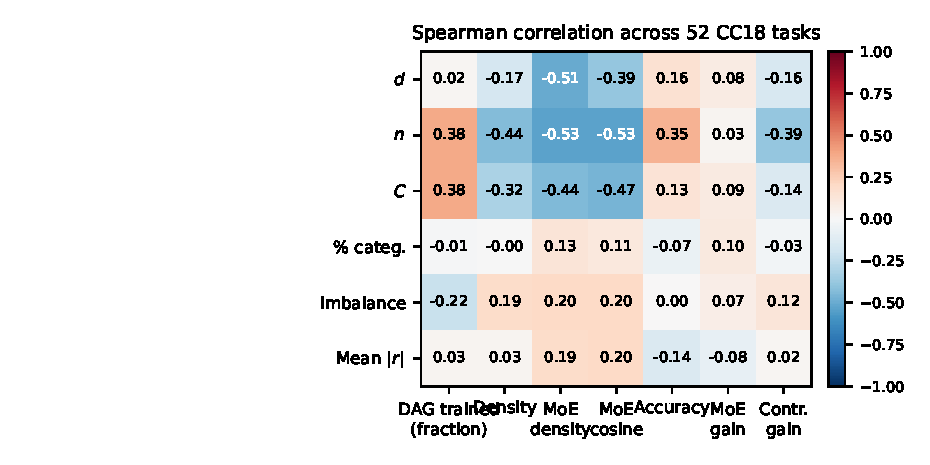
\includegraphics[width=0.85\textwidth]{generated/fig_dag_spearman.pdf}
\caption{Spearman correlations between dataset properties and the learned graphs across \DagN{} CC18 datasets. ``DAG trained'': fraction of the joint phase (routing training) completed at the restored checkpoint. Density is that of $S$ for \Cabin{} and the mean over the $S_k$ for MoE-DAG; gains are relative to \Cabin{} in Table~\ref{tab:cc18}.}
\label{fig:spearman}
\end{figure}




% ============================================================================
\section{Hyperparameters}
\label{app:hyper}

\begin{table}[h]
\centering
\caption{Default configuration of \Cabin{} (all experiments unless stated otherwise) and the origin of each choice. ``Development'': fixed during development, mainly on Dev8 (\S\ref{sec:protocol}), and not tuned afterwards.}
\label{tab:hyper}
\small
\begin{tabular}{@{}L{2.6cm}L{5.6cm}L{6.0cm}@{}}
\toprule
Component & Setting & Origin \\
\midrule
Embedding & VSF, $h=32$, $n_s=2$ slots; categorical: entity embeddings (dim.\ $\le 8$) & development; VSF vs linear embedding in Appendix~\ref{app:design} (D5) \\
Missing values & median imputation + missingness indicators & design study (D5): neutral on average, helps \emph{cylinder-bands} \\
Routing weights & $W=ASA\T$, $k=32$, $A$ row-softmax & design study (D2); $k$ from 4 to 64 within seed noise (Appendix~\ref{sec:sensitivity}) \\
Ordered group graph & VCUDA priorities, $\tau_\pi=0.3$; edges $\tau_E=0.5$ (Gumbel in training, threshold at evaluation) & VCUDA chosen in D3 (no penalty schedule); temperatures: development \\
Sparsity & $\lambda_s=0.05+0.001\,d$ on $S$, joint phase only & development; the $d$ term dates from versions with a $d\times d$ routing matrix \\
Message passing & one round, edge dropout 0.2 & D4 (more rounds hurt); dropout: design study step 3, 0 to 0.3 within noise (Appendix~\ref{sec:sensitivity}) \\
Head & flatten, 2-layer ReLU MLP & development; pooled readouts and target-node readouts hurt (Appendix~\ref{app:negative}) \\
Training & warmup 20 / joint 100 / finetune 30 epochs, batch 32, AdamW (wd $0.01$) & development (end-to-end version, unchanged since) \\
Learning rates & $10^{-3}$ network, $5\cdot10^{-3}$ routing (joint phase), $10^{-4}$ finetune & development \\
Regularization & label smoothing 0.1, gradient clipping 5 & smoothing: design study step 3, 0 to 0.2 within noise; clipping: development \\
Early stopping & 20\% validation split; best validation loss over all phases; patience 25 in finetune & development; restore rule discussed in \S\ref{sec:structure} \\
Ensemble & $M=5$, $\eta=0.1$, adaptive $\alpha$ ($\alpha_0=2$), weight cap 3 & boosting: design study step 4; $M$: Appendix~\ref{sec:sensitivity}; $\eta=0.05$ ties (Appendix~\ref{app:negative}); $\alpha$ and cap: development on 11 datasets \\
Temperature & scalar, L-BFGS on training logits & kept from the original pipeline; does not change predictions \\
\bottomrule
\end{tabular}
\end{table}

% ============================================================================
The boosting strength adapts to the data shape, stronger for high-dimensional data and weaker for many classes:
\[
\alpha=\alpha_0\cdot \mathrm{clip}\!\Big(\frac{\log_2 d}{\log_2 40},0.3,1.2\Big)\cdot \frac{1}{\sqrt{C/2}}\cdot \mathrm{clip}\!\Big(\sqrt{\frac{n}{500}},0.5,1.5\Big),\qquad \alpha_0=2,
\]
and sample weights $w_j=\min(1+\alpha(1-p_{j,y_j}),3)$ are normalized to mean one. (The code also clips from below at 0.5, which never binds since $w_j\ge1$.) The factors were set during development on 11 datasets: high-dimensional datasets benefited from stronger reweighting and multi-class ones from weaker reweighting; the clips avoid extreme values of $\alpha$. In the design study, making $\alpha$ adaptive does not change accuracy (step 5 of Table~\ref{tab:cumulative}). Each numerical feature is embedded by $h_i=\sigma(\mathrm{Lin}_{h\to h}(\sigma(\mathrm{Lin}_{1\to h}(x_i))))$ with ReLU $\sigma$; categorical features use entity embeddings \citep{guo2016entity} projected to the same size.

\section{Additional Results on the Feature Graph}
\label{app:when}

\paragraph{High-dimensional datasets.} The \RealNHigh{} high-dimensional CC18 datasets of \S\ref{sec:when-real} are \RealHighTasks{}.

\paragraph{Estimated graph.} On CC18 the estimated graph has a mean degree of \RealEstDegree{} and takes a median of \RealEstSecondsMedian{}\,s to compute (at most \RealEstSecondsMax{}\,s).

\paragraph{Density-matched controls.}
The controls of \S\ref{sec:when-synth} are frozen random graphs with the same number of edges as the true induced graph (directed, drawn uniformly among ordered pairs) or as the estimated graph (symmetric), expanded to slots like the other graphs, on the full high-dimensional grid ($d\in\{50,100\}$, $n\in\{500,1000\}$, $\lambda\in\{0,1\}$, five SCMs per $d$). Differences in points (SCM as unit, \SynCtrlN{} SCMs):

\begin{center}
\small
\begin{tabular}{@{}lccc@{}}
\toprule
Comparison & all & $\lambda=0$ & $\lambda=1$ \\
\midrule
sparse random (true density) $-$ none & \SynHighRandTrueNone{} & \SynHighRandTrueNoneLamZero{} & \SynHighRandTrueNoneLamOne{} \\
sparse random (est.\ density) $-$ none & \SynHighRandEstNone{} & \SynHighRandEstNoneLamZero{} & \SynHighRandEstNoneLamOne{} \\
sparse random (true density) $-$ dense random & \SynHighRandTrueRandom{} & \SynHighRandTrueRandomLamZero{} & \SynHighRandTrueRandomLamOne{} \\
sparse random (est.\ density) $-$ dense random & \SynHighRandEstRandom{} & \SynHighRandEstRandomLamZero{} & \SynHighRandEstRandomLamOne{} \\
true $-$ sparse random (true density) & \SynHighTrueRandTrue{} & \SynHighTrueRandTrueLamZero{} & \SynHighTrueRandTrueLamOne{} \\
estimated $-$ sparse random (est.\ density) & \SynHighEstRandEst{} & \SynHighEstRandEstLamZero{} & \SynHighEstRandEstLamOne{} \\
additive head: true $-$ sparse random & \SynHighAddTrueRandTrue{} & -- & \SynHighAddTrueRandTrueLamOne{} \\
additive head: estimated $-$ sparse random & \SynHighAddEstRandEst{} & -- & \SynHighAddEstRandEstLamOne{} \\
\bottomrule
\end{tabular}
\end{center}

\paragraph{High-dimensional SCM mechanisms.}
Each edge function of Eq.~\eqref{eq:scm} in the high-dimensional regime is drawn uniformly from $\tanh(ax)$, $bx+(x-b)^2$, $\sin(ax+3b)$, $\max(x-b,0)$, $\exp(-a^2(x-b)^2)$, $\mathbb 1[x>b]$ and $\log(1+|x-b|)$, with $a\sim\mathcal U[0.5,2]$ and $b\sim\mathcal U[-1,1]$ drawn per edge, and each is applied to a standardized output ($z(f_{ji}(x_j))$). If no node has at least two parents and one child, the SCM is redrawn.

\paragraph{\emph{cnae-9}.}\label{sec:when-cnae}
This dataset ($n=1{,}080$, $d=856$) is excluded from Table~\ref{tab:when-real}. On folds 0--2, the original run of Table~\ref{tab:cc18} reaches \CnaeOrig{} and LightGBM \CnaeLgbm{}. The rerun of the routing substitutions failed on folds 1 and 2 because of a fault in the rerun, and we do not report it.

\paragraph{Pooled real-data results.}
Over all \RealPoolN{} datasets (differences averaged over folds before testing), the ensemble with the estimated graph is \RealPoolEnsEstLearned{} points from the default (\RealPoolEnsEstLearnedPe{}) and the ensemble without graph \RealPoolEnsNoneLearned{} (\RealPoolEnsNoneLearnedPe{}). For a single network, the estimated graph is \RealPoolSingleEstLearned{} points above the default (\RealPoolSingleEstLearnedPe{}) but not above no graph (\RealPoolSingleEstNone{}, \RealPoolSingleEstNonePe{}). The single-network differences shrink in the ensemble.

\paragraph{Stochastic gates.}
Part of the failure of the no-graph network on the high-dimensional SCM is an optimization artifact: in \SynHighEarlyRestore{}\% of the runs without graph, the restored checkpoint comes from the first five epochs, and many of these predict a single class. Stochastic gates prevent this collapse, but at $n=500$ and $\lambda=1$ the gated network is still behind LightGBM (\SynHighStgLgbNFiveHundredLamOne{} points). On real data the gates are neutral (\RealStgLearned{} points, dataset-level \RealStgLearnedPe{}; with a weaker penalty \RealStgLThreeLearned{}, \RealStgLThreeLearnedPe{}), hurt on a few low-dimensional datasets (\StgWorst{}), and the single-class collapse is rare, so we do not add them to \Cabin{}.

\paragraph{Interaction measure and heads.}
With the default restore, the correlation across the \RealNLow{} low-dimensional datasets between the interaction proxy and the gain of the default graph under the additive head vanishes ($\rho=\AddLearnedRho{}$), as expected when most returned graphs are untrained. On the \AddNInter{} low-dimensional datasets with an interaction gain above one point, the estimated graph is \RealAddInterEstimatedNone{} points above no graph under the additive head, but this subset is too small for a reliable test. The MLP head without messages is as accurate as the additive head with messages (\RealMlpMinusAddLearned{} points).

\begin{table}[h]
\centering
\caption{Synthetic SCM of Eq.~\eqref{eq:scm} with the additive head, where features can only interact through messages. Same settings as Table~\ref{tab:when-synth}; the additive-head networks use the default restore rule (low-dimensional runs at $n=2{,}000$ used the finetune-only rule and are omitted). \emph{Stumps}: LightGBM restricted to stumps (additive).}
\label{tab:when-add}
\small
\begin{tabular}{@{}lcccccc@{}}
\toprule
Regime & $\lambda$ & None & Dense rand. & True & Estimated & Stumps \\
\midrule
\inputtable{generated/table_struct_synth_add.tex}
\bottomrule
\end{tabular}
\end{table}

\begin{table}[h]
\centering
\caption{Attempts to learn useful routing end to end on the high-dimensional synthetic SCM ($d\in\{50,100\}$, $n=1{,}000$, single network). Accuracy and difference to the true graph with the same head (points). \emph{Finetune restore}: only checkpoints taken after the routing parameters were trained can be restored. \emph{Estimated skeleton}: the edges allowed are those of the two-stage estimated graph. The feature-level DAG was run at $d=100$ only; each $\Delta$ is paired with the reference on the same settings.}
\label{tab:when-e2e}
\small
\begin{tabular}{@{}lcccc@{}}
\toprule
& \multicolumn{2}{c}{$\lambda=0$} & \multicolumn{2}{c}{$\lambda=1$} \\
\cmidrule(lr){2-3}\cmidrule(lr){4-5}
Variant & Acc. & $\Delta$ & Acc. & $\Delta$ \\
\midrule
\inputtable{generated/table_struct_e2e.tex}
\bottomrule
\end{tabular}
\end{table}

% ============================================================================
\section{Negative Results}
\label{app:negative}

Table~\ref{tab:negative} lists the variants tried during development that did not enter the recipe, with the change in mean accuracy against the reference variant of the same benchmark (or of the closest earlier one, marked vA/vB, when the benchmark had no reference of its own). Of the \negNWithData{} variants with surviving results, \negNWorse{} lose at least 0.3 points, \negNNeutral{} are within $\pm0.3$ points and \negNBetter{} gain at least 0.3 points. Variants with small gains were dropped because they did not repeat on other suites or cost more. Several large losses come from a single dataset: multi-round message passing, interleaved message passing and RTDL periodic embeddings collapse on \emph{cnae-9} ($d=856$) and lose only 0.5--0.8 points without it.

{\scriptsize
\setlength{\tabcolsep}{3pt}
\begin{longtable}{@{}L{1.8cm}L{3.4cm}L{0.9cm}L{1.4cm}L{1.6cm}rrL{2.6cm}@{}}
\caption{Negative results of the development study. $\Delta$: mean accuracy difference to the reference (points), over the datasets where both ran ($n$). Suite: development datasets and protocol of the benchmark. Variant names containing ``DAG'' are historical labels from the development logs; the final model uses the ordered routing of \S\ref{sec:method}.}\label{tab:negative}\\
\toprule
Dimension & Variant & Version & Reference & Suite & $\Delta$ & $n$ & Conclusion \\
\midrule
\endfirsthead
\toprule
Dimension & Variant & Version & Reference & Suite & $\Delta$ & $n$ & Conclusion \\
\midrule
\endhead
\bottomrule
\endfoot
\inputtable{generated/table_negative.tex}
\end{longtable}
}

% ============================================================================
\section{Per-Dataset Results}
\label{app:perdataset}

\begin{table}[h]
\centering
\caption{Accuracy (5-fold mean) of every method on the \NCCtasks{} CC18 datasets of Table~\ref{tab:cc18}. Best per dataset in bold.}
\scriptsize
\setlength{\tabcolsep}{2.5pt}
\begin{tabular}{@{}lrrr*{10}{c}@{}}
\toprule
Dataset & $n$ & $d$ & $C$ & \inputtable{generated/table_per_dataset_header.tex} \\
\midrule
\inputtable{generated/table_per_dataset.tex}
\bottomrule
\end{tabular}
\end{table}

% ============================================================================
\section{Reproducibility}
\label{app:repro}

Every number, table and figure in this paper is generated from the result files by a single script; no number is typed by hand. The model code, the benchmark harness and all per-fold results are available at \CodeURL{}. The new runs (synthetic recovery, DAG extraction, sensitivity) fix the random seed.

\end{document}
